\documentclass[11pt,a4paper]{article}

\usepackage[margin =1 in]{geometry}
\usepackage[none]{hyphenat}
\usepackage{amsmath,amsfonts}
\usepackage{amssymb}
\usepackage{graphicx}
\usepackage{multirow}
\usepackage{float}
\usepackage{tikz}
\usepackage{color}
\usepackage{xcolor}

% ---------------------------------------------------------------------------
% Additions for the web build; nothing here changes the printed page.
% enumitem preserves the optional label on \item[(a).], which tex4ht otherwise
% discards and renumbers.
% ---------------------------------------------------------------------------
\usepackage{enumitem}
\usepackage{amsthm}
\theoremstyle{definition}
\newtheorem{thm}{Theorem}[section]
\newtheorem{definition}[thm]{Definition}
\newtheorem{example}[thm]{Example}
\newtheorem{note}[thm]{Note}
\newtheorem{remark}[thm]{Remark}
% No provenance label on problems: these are practice problems, not a
% reproduction of any one course's assessment.
\newtheorem{problemx}{Problem}[section]
\newenvironment{problem}{\begin{problemx}}{\end{problemx}}
\newenvironment{solution}
  {\renewcommand{\qedsymbol}{}\begin{proof}[\textit{Solution}.]}
  {\end{proof}}




\usetikzlibrary{graphs,patterns,arrows.meta,fadings,shapes,trees,bending,angles,quotes}



\parindent 0ex

\begin{document}
% Title page depersonalised for the web, as with every other course here:
% no university, no lecturer, no year. The identity below is kept - it is the
% two forms of the Kruskal-Wallis statistic, and it says what the course is
% about better than a subtitle would.
\begin{titlepage}
\begin{center}
\vspace*{3cm}
{\Huge\bfseries Methods of Non-Parametric Statistics}\\[1.2cm]
{\large Lecture Notes}\\[2.5cm]
\line(1,0){300}\\[1.5cm]
$$\frac{12}{N(N+1)}\sum^k_{i=1}\frac{1}{n_i}
\Bigg[R_i-\frac{n_i(N+1)}{2}\Bigg]^2
=\frac{12}{N(N+1)}\sum^k_{i=1}\frac{R^2_{i}}{n_i}-3(N+1)$$
\end{center}
\end{titlepage}

\tableofcontents
\thispagestyle{empty}
\clearpage
\setcounter{page}{1}









\textbf{Rationale}
\hrulefill\\

The parametric statistical methods depend so much on the underlying distributions of the random variable and independence of measurements. However there are many situations when the assumption of the underlying distribution and or independence do not hold. Non-parametric statistical methods are then required. This course gives students techniques and skills to perform some non-parametric procedures.\\








\textbf{Objectives}\\ At the end of the course, students should be able to :-
\begin{enumerate}
\item Explain the difference between non-parametric and parametric procedures.
\item Perform some statistical tests based on Binomial distributions (Binomial test, Quantile test).
\item Perform some statistical tests based on ranks for one sample, two samples, one-way ANOVA and two-way ANOVA.
\item Perform goodness of fit tests.\\
\end{enumerate}




\textbf{Pre-requisites:} Mathematical Statistics and Analysis and Design of Experiments.\\







\pagebreak
\textbf{Course Content}
\hrulefill\\
\begin{enumerate}
\item \textbf{Introduction}\\ 
Populations, samples and statistics. Estimation. Hypothesis testing. Some properties of hypothesis tests. Some comments on non-parametric statistics.
\item \textbf{Some test based on Binomial Distribution}\\ 
Binomial test. Quantile test. Sign test and its variations.
\item \textbf{Some tests based on Ranks}\\ 
One and two independent samples. Several independent samples, Kruskal-Wallis one-way analysis of variance. Friedman two-way analysis of variance. The one-sample or matched-pairs case. Measures of rank correlation.
\item \textbf{Statistics of Kolmogorov-Smirnov type}\\ 
The Kolmogorov goodness-of-fit test. Tests on two independent samples. Tests on several independent samples.\\\\
\end{enumerate}










\pagebreak

\section{\textbf{INTRODUCTION}}

This chapter surveys the ideas the rest of the course depends on. One point should
be settled before anything else, because the name misleads almost everybody who
meets it first:

\begin{note}
It is the \emph{method} that is non-parametric, not the data. Nothing about a data
set makes it non-parametric; what is non-parametric is a procedure that does not
require the population to belong to a specified family of distributions.
\end{note}

\subsection{Parametric Inference, Recalled}

Parametric and non-parametric are the two broad classifications of statistical
procedure. A parametric procedure assumes the observations come from a distribution
of known form, indexed by finitely many unknown parameters, and draws its
conclusions about those parameters.

\textbf{The normal distribution.} The best known family is the normal, indexed by
the mean $\mu$ and variance $\sigma^{2}$. Given independent observations from it,
the sample mean $\overline{X}$ is a point estimate of $\mu$; the $t$-test measures
the strength of evidence against an \emph{a priori} hypothesised value $\mu_0$; and
a confidence interval gives a range of plausible values for the true mean. All of
this is parametric inference, and all of it leans on the assumed normality.

The normal distribution is strictly appropriate only to certain continuous
measurements, though it often works well enough when the measurement scale is fine
and the distribution roughly symmetric.

\textbf{The binomial distribution.} For counts, the binomial family has parameters
$n$, the number of observations, and $P$, the probability that the event of
interest occurs at any one of them. The number of occurrences $R$, with
$0 \leq R \leq n$, satisfies
$$P(R = r) = \binom{n}{r}P^{r}(1-P)^{\,n-r},$$
and $\widehat{P} = r/n$ is the point estimate of $P$. Again one may test an
\emph{a priori} value $P_0$ or form a confidence interval.

The binomial is relevant to counts in discrete outcome situations --- the number of
males in a family of size $n$, for instance. The outcome being counted is
conventionally called the ``favourable'' event, a name that sits awkwardly when the
event is a positive diagnosis of an illness.

\textbf{Other families.} Uniform, multinomial, Poisson, exponential, double
exponential, gamma and many others. Sometimes theory or experience makes it
reasonable to assume a particular family; often it does not.

\subsection{When Parametric Inference Will Not Do}

\begin{enumerate}
\item[(i).] The assumption may be unreasonable. Examination marks, for example,
are bounded and frequently skewed, and no standard family fits them naturally.
\item[(ii).] Even with precise measurements, assuming normality asserts properties
--- symmetry, unbounded support, specific tail behaviour --- that the data may
visibly contradict.
\item[(iii).] The data may not be measurements at all. For ranked or ordered
categorical data there is no numerical scale on which a mean is meaningful.
\end{enumerate}

\begin{definition}
A statistical method is \emph{distribution-free} if the null distribution of its
test statistic does not depend on the distribution from which the sample was
drawn.
\end{definition}

\begin{note}
``Distribution-free'' and ``non-parametric'' are used interchangeably, and the term
is slightly misleading in the same way the first note warned about. It does
\emph{not} say the test statistic has no distribution --- it has a perfectly
definite one. It says the method may be applied whatever the population
distribution happens to be.
\end{note}

Non-parametric methods make weaker assumptions, but they are not preferred in all
situations. Breadth of applicability is bought at a price: when a parametric
assumption is justified, the parametric test extracts more information from the
same data and is more powerful. The sensible rule is to use the parametric method
when its assumptions hold and the non-parametric one when they do not.

Most of the tests here concern measures of \emph{location} --- the mean, and more
often the median --- though measures of \emph{dispersion} such as the variance and
standard deviation also arise.

\subsection{Population and Sample}

\begin{definition}
A \emph{random sample} of size $n$ from a distribution is a sequence
$X_1, \ldots, X_n$ of independent observations, each having that distribution.
\end{definition}

Independence means that knowing one value tells us nothing about the others. It is
the requirement most often violated in practice and the one whose violation does
most damage --- Chapter 6 returns to exactly this point for time-ordered data.

In practice we rarely sample from a cleanly specified distribution. If a new diet
is tested on twenty pigs at one agricultural station, the twenty are not a random
sample from all pigs; they are the pigs available. The population being sampled is
then a hypothetical one, and the inference is only as good as that idealisation.

\subsection{Hypothesis Tests, Recalled}

To test a hypothesis about the unknown mean $\mu$ of a normal distribution we
specify a null hypothesis $H_0 : \mu = \mu_0$, compute the statistic $t$ from the
sample, and compare $\left|t\right|$ with a tabulated critical value
$t_{\alpha}$.

If $\left|t\right| \geq t_{\alpha}$ the result is called \emph{significant at
level} $\alpha$, and we \emph{reject} $H_0$. Conventional levels are
$\alpha = 0.05$, $0.01$ and $0.001$, described as significant, highly significant
and very highly significant.

\begin{note}
\textbf{What significance does and does not mean.} If the result is not
significant we \emph{fail to reject} $H_0$; we do not accept it, and we certainly
do not conclude that it is true. Failing to detect a difference is not the same as
demonstrating there is none --- a small sample will fail to reject almost any null
hypothesis.

Nor does significance establish that $H_0$ is false. It says the data would be
unusual if $H_0$ held, and at $\alpha = 0.05$ one test in twenty will say so when
$H_0$ is perfectly true. This is the single most common misreading of a
significance test, and Chapter 6 shows what it costs when two hundred tests are
run at once.
\end{note}

\subsection{The Rationale of $H_0$ and $\alpha$}

If $H_0$ is true, values of $t$ near zero are more likely than large ones of either
sign; if $H_0$ is false, large $\left|t\right|$ becomes more likely. Choosing
$\alpha = 5\%$ means that over many independent tests performed when $H_0$ is true,
about one in twenty will be declared significant. That is the rate of false
positives we agree to tolerate.

Modern software reports the exact probability of a value at least as extreme as the
one observed --- the $P$-value --- and $H_0$ is rejected when
$P \leq \alpha$, which is the same rule as $\left|t\right| \geq t_\alpha$.

\begin{definition}
A \emph{Type I} error is rejecting $H_0$ when it is true; its probability is
$\alpha$. A \emph{Type II} error is failing to reject $H_0$ when it is false; its
probability is denoted $\beta$. The \emph{power} of the test is $1 - \beta$, the
probability of detecting a departure from $H_0$ when one exists.
\end{definition}

Large power is desirable, and it is precisely where non-parametric tests pay for
their generality: against normal data the sign test has markedly less power than
the $t$-test, while against skewed or contaminated data it may have more.

\subsection{Types of Hypotheses}

The choice of $H_1$ is determined by the logic of the problem, not by the data.
\begin{enumerate}
\item[(i).] \emph{Two-tailed}: $H_0 : \mu = \mu_0$ against
$H_1 : \mu \neq \mu_0$, when a departure in either direction matters.
\item[(ii).] \emph{One-tailed}: $H_0 : \mu = \mu_0$ against
$H_1 : \mu > \mu_0$ (or $<$), when only one direction is of interest and the other
would be treated as no effect.
\end{enumerate}
Choosing one tail after seeing which way the data fell doubles the true error rate
and is not legitimate.

\subsection{A First Non-Parametric Test}

Some non-parametric statistics have approximately continuous null distributions,
the normal among them; others are frankly discrete, and the following is one.

\begin{example}
Survival times are recorded for ten patients. Test
$$H_0 : \theta = 200 \qquad\text{against}\qquad H_1 : \theta \neq 200$$
at the $5\%$ level, where $\theta$ is the population median. Suppose three of the
ten observations exceed $200$.

\textbf{The statistic.} Count the observations above $200$, recording each as a
``$+$''. By the definition of the median, under $H_0$ each observation is above
$200$ with probability $\tfrac12$, independently. So the number $R$ of ``$+$''
signs satisfies
$$R \sim B\!\left(10, \tfrac12\right),
\qquad
P(R = r) = \binom{10}{r}\left(\tfrac12\right)^{10}.$$

\textbf{The null distribution.}
\begin{center}
\begin{tabular}{c|ccccccccccc}
$r$ & 0 & 1 & 2 & 3 & 4 & 5 & 6 & 7 & 8 & 9 & 10\\
\hline
$P(R=r)$ & $0.0010$ & $0.0098$ & $0.0439$ & $0.1172$ & $0.2051$ & $0.2461$
& $0.2051$ & $0.1172$ & $0.0439$ & $0.0098$ & $0.0010$\\
\end{tabular}
\end{center}
The distribution is symmetric about $r = 5$, as it must be when $P = \tfrac12$.

\textbf{The test.} With $R = 3$ observed, the evidence against $H_0$ in the lower
tail is
$$P(R \leq 3) = \sum^{3}_{r=0}\binom{10}{r}\left(\tfrac12\right)^{10}
= \dfrac{1+10+45+120}{1024} = \dfrac{176}{1024} = 0.1719 .$$
The alternative is two-sided, and by symmetry $P(R \geq 7) = P(R \leq 3)$, so
$$P\text{-value} = 2(0.1719) = 0.3438 .$$

\textbf{Decision.} Since $0.3438 > 0.05$ we do not reject $H_0$. There is no
evidence at the $5\%$ level that the median differs from $200$.
\end{example}

\begin{note}
Three out of ten looks like a clear imbalance and is not. With only ten
observations the sign test cannot resolve anything but a gross departure: even
$R = 1$ gives a two-sided $P$-value of $2(0.0108) = 0.0215$, and $R = 2$ gives
$0.1094$. The test is honest about how little ten signs can tell us --- which is
the point of computing the null distribution rather than trusting the impression.
\end{note}

\section{\textbf{SOME TESTS BASED ON BINOMIAL DISTRIBUTION}}

\begin{enumerate}
\item[-] A random variable $X$, a count of the occurrences of some outcome in a fixed number of observations $(n)$ is Binomial if 
\begin{enumerate}
\item[*] each observation falls into one of the just two categories i.e success/failure.
\item[*] $n$ observations are all independent.
\item[*] probability of success is the same for each observations
\end{enumerate}
$X\thicksim B(n,P)$
\item[-] Sign and Binomial tests are examples of NP tests that are based on the Binomial distribution.\\\\
\end{enumerate}








\subsection{Sign Test}

\begin{definition}
Let $X_1, X_2, \ldots, X_n$ be a random sample from a continuous distribution with
median $M$. The \emph{sign test} of
$$H_0 : M = M_0 \qquad\text{against}\qquad H_1 : M \neq M_0$$
discards every observation equal to $M_0$, replaces each of the remaining $n'$
observations by the sign of $X_i - M_0$, and bases the decision on
$$N_{+} = \#\{i : X_i > M_0\},
\qquad
N_{-} = \#\{i : X_i < M_0\},
\qquad N_{+} + N_{-} = n' .$$
\end{definition}

The test uses only the \emph{signs} of the deviations, never their sizes. That is
its strength and its weakness at once: no assumption about the shape of the
distribution is needed, but a great deal of information is thrown away, and where
the Wilcoxon signed-rank test is applicable it will usually be preferred.

\begin{thm}
Under $H_0$ the sign statistic is binomial,
$$N_{+} \ \sim\ B\!\left(n', \tfrac12\right),$$
so that $E(N_{+}) = \dfrac{n'}{2}$ and
$\operatorname{var}(N_{+}) = \dfrac{n'}{4}$.
\end{thm}

\begin{proof}
Since the distribution is continuous, $P(X_i = M_0) = 0$ and each retained
observation satisfies $P(X_i > M_0) = P(X_i < M_0) = \tfrac12$ under $H_0$, by the
definition of the median. The observations are independent, so $N_{+}$ counts the
successes in $n'$ independent trials each of probability $\tfrac12$.
\end{proof}

\begin{note}
\textbf{Paired data.} For matched pairs $(Y_i, Z_i)$ the test is applied to the
differences $X_i = Y_i - Z_i$ with $M_0 = 0$, giving a distribution-free
alternative to the paired $t$-test. For a single sample it replaces the one-sample
$t$-test, and for ordered categorical data --- where a numerical scale is
inappropriate but observations can be ranked --- it is often the only test
available.
\end{note}

\textbf{Test procedure.} Choose whichever of $N_{+}$, $N_{-}$ the alternative
makes appropriate, and compute the exact binomial tail probability with
$p = \tfrac12$:
\begin{enumerate}
\item[(i).] for a one-sided alternative, that tail probability is the $P$-value;
\item[(ii).] for a two-sided alternative, double it.
\end{enumerate}

\begin{thm}[Large-sample approximation]
Let $R = \min\left(N_{+}, N_{-}\right)$. For $n' \geq 25$ the standardised
statistic
$$Z = \dfrac{n' - 2R - 1}{\sqrt{n'}}$$
is approximately standard normal under $H_0$, and $H_0$ is rejected at level
$\alpha$ when $Z > Z_{\alpha/2}$ for a two-sided test.
\end{thm}

\begin{proof}
By the previous theorem $N_{+} \sim B(n',\tfrac12)$, so the standardised variable
is
$$\dfrac{N_{+} - n'/2}{\sqrt{n'/4}} = \dfrac{2N_{+} - n'}{\sqrt{n'}} .$$
Taking $R$ to be the smaller count and applying the continuity correction of
$\tfrac12$ towards the mean replaces $2R - n'$ by $2R + 1 - n'$, and changing sign
so that the statistic is positive gives
$$Z = \dfrac{n' - 2R - 1}{\sqrt{n'}} .$$
Equivalently, since $N_{+} + N_{-} = n'$ gives
$\left|N_{+} - N_{-}\right| = n' - 2R$,
$$Z = \dfrac{\left|N_{+}-N_{-}\right| - 1}{\sqrt{n'}} ,$$
which is the form quoted in many texts.
\end{proof}

\begin{note}
\textbf{$R$ must be the smaller of the two counts.} If the larger is used, $Z$
comes out negative and the test is mis-signed --- with $n' = 30$ and the counts
$20$ and $10$, the correct value is $Z = 1.643$ and the wrong choice gives
$-2.008$.

The approximation is good well before $n' = 25$. At $n' = 30$ with $R = 10$ it
returns a two-sided $P$-value of $0.1004$ against the exact binomial $0.0987$; at
$n' = 60$ with $R = 22$, $0.0528$ against $0.0519$. When the decision is close to
the boundary, use the exact binomial.
\end{note}
\textbf{Tied Scores}
\begin{enumerate}
\item[-] If a subject has the same score in each condition, there will be no sign, because the difference score is zero.
\item[-] Two methods of handling zero difference are proposed.
\begin{enumerate}
\item Scores are dropped from the sample and reduced $n$ by the appropriate number.
\item It may not be the best way as can lead to loss of too much power.
\end{enumerate}

\item[-] Best practice is that 
\begin{enumerate}
\item[*] if one observation/score/subject with tied score drop that subject.
\item[*] if two subjects with tied score, make one a "$+$" and one a "$-$".
\item[*] generally for odd number of subject $(>1)$ drop one randomly selected subject and then proceed as for even numbered tied scores.\\\\ 
\end{enumerate}
\end{enumerate}








\textbf{Example 1}\\
A random sample of 10 students weight (Kg) from student population is given as $$135\,,\, 119\,,\, 106\,,\, 135\,,\, 180\, ,\,108\,,\, 128\,,\, 160\,,\, 143\,,\, 175$$ 
Find out as as whether the median weight of students population is different from 140 Kg. Using the sign test $$H_0:\theta =140\hspace{0.5cm} \text{vs}\hspace{0.5cm} H_1:\theta \neq 140$$ 

$$-\hspace{0.3cm}-\hspace{0.3cm}-\hspace{0.3cm}-\hspace{0.3cm}+\hspace{0.3cm}-\hspace{0.3cm}-\hspace{0.3cm}+\hspace{0.3cm}+\hspace{0.3cm}+$$ $$N_+=4,\hspace{1cm}N_+\thicksim B\Big(10,\frac{1}{2}\Big)$$ 

$$\text{C.R}\hspace{0.5cm} 4\hspace{0.4cm}\text{and}\hspace{0.4cm} 6$$ $$P(N_+\leq 4)\cup P(N_+\geq 6)$$

\begin{align*}
P-\text{value} &=P(N_+\leq 4)+P(N_+\geq 6)\\
               &=2P(N_+\leq 4)\hspace{1cm}\text{by symmetry}\\\\
               &=2\sum^4_{i=0}C_i^{10}\Big(\frac{1}{2}\Big)^{10}\\
               &=2(0.376953125)\\
               &=0.754\\
\end{align*}











\textbf{Example 2}\\
A psychologist want to know if monkeys prefer stimulation of brain area A to train area B. In the experiment 14 monkeys are taught to press two  bars. When a light comes on, presses for 1 always result in simulation of area A; presses on bars 2 always result in simulation of area B.\\After learning to pass the bars, the monkeys are tested for 15 months, during which time the frequencies for two bars are recorded. The data is shown.

\begin{table}[H]
\centering
\begin{tabular}{c|c|c}
Bar 1&Bar 2& Sign of the\\
&&dev(1-2)\\
\hline 20&40&-\\
18&25&-\\
24&38&-\\
14&27&-\\
5&31&-\\
26&21&+\\
15&32&-\\
29&38&-\\
15&25&-\\
9&18&-\\
25&32&-\\
31&28&+\\
35&33&+\\
12&29&-\\
\end{tabular}
\end{table}

Find out whether there is a difference in the two conditions at $5\%$ level of significance.\\



Sign test.\\


\textit{Formulation and assumptions}\\ 
The researcher did not predict a particular outcome but wanted to know if the two conditions differ. There it is non directional i.e\\

$H_0$: No differences between frequencies.\\ $H_1$: frequencies differ , 2-sided.\\

$\therefore$ Extreme number of `$+$' signs, smaller or large will support $H_1$. A middling number of `$+$' signs would be consistent with $H_0$.\\\\ 






\textit{Procedure}
\begin{enumerate}
\item[-] Sampling distribution of the test statistic is the Binomial distribution with $N=14$ and $P=0.5$ i.e $\Big(14,\dfrac{1}{2}\Big)$.
\item[-] To carry out the sign test consider $$S_+=3\hspace{0.5cm}\text{and}\hspace{0.5cm} S_-=11$$ 

$$N=\min(S_+,S_-)=3$$ $$N=3\hspace{1cm}\text{is}\hspace{0.3cm}+\hspace{0.3cm}\text{Signs}$$

\item[-] Since $H_1$ is non directional/ 2-sided we must find $$P(N\leq 3)+P(N\geq 11)$$ $$\text{C.V}:\hspace{0.5cm} 3\hspace{1cm} \text{and}\hspace{1cm} 11$$ 

$$\text{C.R}\hspace{0.5cm} N\leq 3\hspace{0.5cm}\text{and}\hspace{0.5cm}N\geq 11$$
\begin{align*}
P-\text{value} &=P(N\leq 3)+P(N\geq 11)\\
               &=0.029+(1-P(N<11))\\
               &=1.029-0.971\\
               &=0.0578
\end{align*}
\textit{Conclusion:}\\ No sufficient evidence to allow the rejection of $H_0$.\\\\
\end{enumerate}












\textbf{Example}:\\ 
17 teachers attend a summer school to improve their listening skills. They were given a pretest and potest: 16 teachers improved, 1 did more poorly.\\
Did participation improve their performance on listening test? $\theta=0.05$\\\\




\subsection{C.I for Median Based on Sign Test}
\begin{enumerate}
\item[-] $M_L$ will denote the lower limit.
\item[-] $M_U$ will denote the upper limit.
\item[-] Two methods for constructing interval estimate of unknown population median are
\begin{enumerate}
   \item[*] based on sign test.
   \item[*] based on  Wilcoxon test.\\\\
\end{enumerate}
\end{enumerate}









\pagebreak
\subsection{To Solve C.I for Median Based on Sign Test}



\textbf{Small Sample Sizes}
\begin{enumerate}
\item[-] Arrange the order of data given according to the values.
\item[-] Find the cumulative probabilities from Binomial tables or build your own table.
\item[-] Find $K'$ (position).
\item[-] Calculate both C.I by using $100(1-2\alpha)\%$.
\item[-] Determine the $(K'+1)^{th}$ value in the ordered array as $M_L$ and $(n-K')^{th}$ value in the ordered array as $M_U$.
\item[-] Make conclusion.\\\\
\end{enumerate}






\textbf{Large Sample Approximation $(n>25)$}
\begin{enumerate}
\item[-] Arrange the ordered data given according to the values.
\item[-] Find $K'+1$ by using \hspace{0.2cm}$\displaystyle{K'+1\thickapprox \frac{n}{2}-Z_{\frac{\alpha}{2}}\sqrt{\frac{n}{4}}}$
\item[-] Determine the $(K'+1)^{th}$ value in the ordered array as $M_L$ and $(n-K')^{th}$ values in the ordered array as $M_U$.
\item[-] Make conclusion.\\\\
\end{enumerate}











\textbf{Example: Small Sample size}\\ 
A study of side effects of drugs reported data shown in the table below. $$4.0,\hspace{0.3cm} 3.0,\hspace{0.3cm} 7.0,\hspace{0.3cm} 5.4,\hspace{0.3cm} 3.8,\hspace{0.3cm} 10.0,\hspace{0.3cm} 7.3,\hspace{0.3cm} 2.6,\hspace{0.3cm} 1.8,\hspace{0.3cm} 7.5$$
Construct a $95\%$ C.I for $\theta$ of the population from which the sample data have been drawn.\\\\




\textbf{Solution:}
\begin{enumerate}
\item Arrange data in ascending order $$1.8,\hspace{0.3cm} 2.6,\hspace{0.3cm} 3.0,\hspace{0.3cm} 3.8,\hspace{0.3cm} 4.0,\hspace{0.3cm} 5.4,\hspace{0.3cm}7.0,\hspace{0.3cm} 7.3,\hspace{0.3cm} 7.5,\hspace{0.3cm} 10.0$$
\item Determine the amount sample (sample size) $n=10$: $n<25$ small sample size.
\item \hspace{0.3cm}

\begin{figure}[H]
\centering
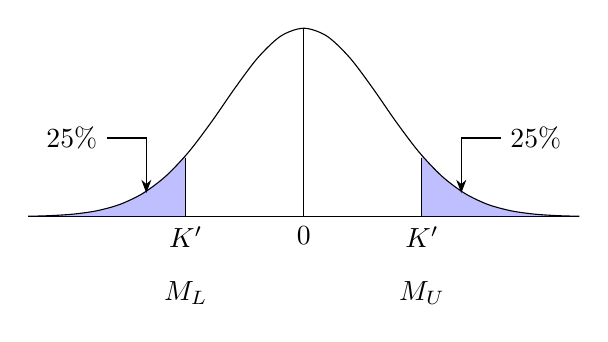
\begin{tikzpicture}
\draw(-3.5,0)--(3.5,0)
(0,0)--(0,2.39);
\path[fill=blue,opacity=0.25, smooth, domain=1.5:3.5,variable=\x]plot(\x,{6*1/sqrt(2*pi)*exp(-1/2*\x*\x)})--(3.5,0)--(1.5,0)--(1.5,0.75);
\path[fill=blue,opacity=0.25, smooth, domain=-3.5:-1.5, variable=\x]plot(\x,{6*1/sqrt(2*pi)*exp(-1/2*\x*\x)})--(-1.5,0.75)--(-1.5,0)--(-3.5,0);
\draw[smooth,domain=-3.5:3.5,variable=\x]plot(\x,{6*1/sqrt(2*pi)*exp(-1/2*\x*\x)});
\draw(1.5,0.75)--(1.5,0)
(-1.5,0)--(-1.5,0.75);
\draw(-1.5,0)node[below]{$K'$}
(1.5,0)node[below]{$K'$}
(0,0)node[below]{0}
(-1.5,-0.7)node[below]{$M_L$}
(1.5,-0.7)node[below]{$M_U$}
(2.5,1)node[right]{$25\%$}
(-2.5,1)node[left]{$25\%$};
\draw[-Stealth](2.5,1)--(2,1)--(2,0.3);
\draw[-Stealth](-2.5,1)--(-2,1)--(-2,0.3);
\end{tikzpicture}
\end{figure}


Referring to the question we want to construct $95\%$ C.I. Thus, we need to find $K'$ as observation value.\\ 
Value of $K'$ will be referred by cumulative of probability distribution of Binomial distribution as $$P(K\leq A| n,P)=B$$ $$\implies \hspace{0.3cm} P(K\leq 1 | 10,1/2)=0.0108$$ $$\implies \hspace{0.3cm} P(K\leq 2 | 10,1/2)=0.0547$$ We choose $K'=1$ and $K'=2$ as observation values. This is because we need to construct the first case and second  case.\\
\end{enumerate}







1$^{st}$: The Wider Interval.\\
Let $K'=1$, with cumulative probability 0.0108$$\implies \hspace{0.4cm} 100(1-2\alpha)=100(1-2(0.0108))=97.89\%\hspace{0.3cm}\text{C.I}$$ The amount of cumulative probability should be less than 0.05 as significant value. Choose interval is wider and higher of C.I.\\


2$^{nd}$: The narrow interval and lower C.I let $K'=2$ and cumulative probability 0.0541 $$\implies \hspace{0.4cm} 100(1-2(0.0547))=89.06\%\hspace{0.3cm} \text{of C.I}$$\\





\textbf{Note:}\\ The amount of cumulative probability should be more than 0.05 as significant value because the chosen interval is narrow and lower of C.I $$P(K'\leq 1 |10,1/2)=0.0108\hspace{0.8cm} \text{and}\hspace{0.8cm} P(K'\leq 2|10,1/2)=0.0547.$$ For the 1$^{st}$ and 2$^{nd}$ cases, we will find the upper and lower limit as:\\\\



\textit{Case 1:}\\
$K'=1,\implies K'+1=2$\\
Thus, the observation is second observation from such ends of the ordered array  yields as below



\begin{table}[H]
\centering
\begin{tabular}{cccccccccc}
1.8&2.6&3.0&3.8&4.0&5.4&7.0&7.3&7.5&10\\
1&(2)&3&4&5&6&7&8&(9)&10\\
\end{tabular}
\end{table}


Therefore $\hspace{0.6cm} M_L=2.6;\hspace{0.4cm} M_U=7.5$\\


$\implies$ C.I for $\theta$ is $(2.6,7.5)$ with $97.84\%$ confidence.\\


\textit{Case 2:}\\
$K'=2\implies K'+1=3$.\\

$\implies \hspace{0.4cm} M_L=3.0;\hspace{0.4cm} M_U=7.3$\\


$\implies \hspace{0.4cm} 89.06\%$ C.I for $\theta$ is $(3.0,7.3)$\\\\\








\textbf{Example: Large Sample}\\ 
In a study of sleep patterns the data was collected and received. Percentage of total sleep time 16 mentally and physically health males  between the ages 50-60.
\begin{table}[H]
\centering
\begin{tabular}{cccccccc}
1.90&3.08&9.10&3.53&1.99&3.10&10.16&0.69\\
1.74&2.41&4.01&3.71&8.11&8.23&0.07&3.07\\
\end{tabular}
\end{table}


Construct a $95\%$ C.I for median from the sample data.\\


1$^{st}$: Arrange data in ascending orders.\\



2$^{nd}$: Determine sample size. We use the large sample approximation given by $$K'+1\thickapprox \frac{n}{2}-Z_{\frac{\alpha}{2}}\sqrt{\frac{n}{4}}$$
C.I $\hspace{0.5cm}95\%\hspace{1.2cm} \alpha =0.05$ $$Z_{\frac{\alpha}{2}}=Z_{0.025}=1.96$$ $n=16\implies K'+1\thickapprox 4$\\ 


Considering 4 observations from each end of the ordered array $M_L=1.90$ and $M_U=8.11$\\ 

$95\%$ C.I is between 1.90 and 8.11.\\

















\pagebreak
\section{\textbf{SOME TESTS BASED ON RANKS}}



\subsection{Wilcoxon Signed Rank Test}

The sign test throws away the sizes of the differences and keeps only their signs.
The Wilcoxon signed-rank test keeps a little more --- the \emph{order} of the
sizes --- and is correspondingly more powerful.

\begin{definition}
Let $(Y_i, Z_i)$, $i = 1,\ldots,n$, be matched pairs and put $d_i = Y_i - Z_i$.
Discard every pair with $d_i = 0$, leaving $n'$ pairs. Rank the remaining
$\left|d_i\right|$ from $1$ to $n'$, smallest first, assigning \emph{average
ranks} to ties. The \emph{signed-rank statistics} are
$$T_{+} = \sum_{d_i > 0}\operatorname{rank}\left|d_i\right|,
\qquad
T_{-} = \sum_{d_i < 0}\operatorname{rank}\left|d_i\right|,$$
and necessarily
$$T_{+} + T_{-} = \dfrac{n'(n'+1)}{2}.$$
\end{definition}

The identity is a useful arithmetic check: the two statistics must add to the sum
of the first $n'$ integers, because every retained pair contributes its rank to
exactly one of them.

\begin{example}
Two treatments are compared on eight subjects.

\begin{center}
\begin{tabular}{c|c|c|c|c|c}
Obs & Sample 1 & Sample 2 & $d = S_1-S_2$ & $\left|d\right|$ & Rank of $\left|d\right|$\\
\hline
1 & 9  & 8  & $+1$ & 1 & $2$\\
2 & 6  & 9  & $-3$ & 3 & $5$\\
3 & 8  & 10 & $-2$ & 2 & $4$\\
4 & 7  & 7  & $0$  & --- & discarded\\
5 & 10 & 6  & $+4$ & 4 & $6$\\
6 & 5  & 4  & $+1$ & 1 & $2$\\
7 & 6  & 5  & $+1$ & 1 & $2$\\
8 & 7  & 7  & $0$  & --- & discarded\\
\end{tabular}
\end{center}

Two pairs are discarded, so $n' = 6$. The absolute differences in order are
$$1,\ 1,\ 1,\ 2,\ 3,\ 4 .$$
The three $1$'s would occupy ranks $1, 2, 3$; being tied they each receive the
average $\frac{1+2+3}{3} = 2$. The remaining values take ranks $4$, $5$, $6$.

\begin{center}
\begin{tabular}{l|cccccc}
$\left|d\right|$ sorted & 1 & 1 & 1 & 2 & 3 & 4\\
\hline
Provisional rank & 1 & 2 & 3 & 4 & 5 & 6\\
Rank used (ties averaged) & $2$ & $2$ & $2$ & $4$ & $5$ & $6$\\
Sign of $d$ & $+$ & $+$ & $+$ & $-$ & $-$ & $+$\\
\end{tabular}
\end{center}

Hence
$$T_{+} = 2 + 2 + 2 + 6 = 12,
\qquad
T_{-} = 4 + 5 = 9,$$
and the check holds: $12 + 9 = 21 = \dfrac{6(7)}{2}$.
\end{example}

\begin{note}
\textbf{Ties must be averaged, even when it seems not to matter.} In this example
the provisional ranks $1,2,3$ would give $T_{+} = 1+2+3+6 = 12$ as well, because
all three tied observations happen to be positive and $1+2+3 = 3 \times 2$. That
is a coincidence of this data set and not a licence: had one of the three been
negative, the two rankings would have disagreed. Average the ranks always.
\end{note}

\textbf{Hypotheses and the matching statistic.} Write $D_1$, $D_2$ for the two
distributions. The statistic to use is the one that becomes \emph{small} under the
alternative:

\begin{center}
\begin{tabular}{l|l|l}
Alternative & Statistic & Reject $H_0$ when\\
\hline
$D_1$ shifted \emph{left} of $D_2$ & $T_{+}$ & $T_{+} \leq T_0$\\
$D_1$ shifted \emph{right} of $D_2$ & $T_{-}$ & $T_{-} \leq T_0$\\
$D_1$ shifted either way & $T = \min(T_{+},T_{-})$ & $T \leq T_0$\\
\end{tabular}
\end{center}

\begin{note}
The pairing is worth pausing over, because it is easy to get backwards. If $D_1$
lies to the \emph{left} of $D_2$ then the differences $d = S_1 - S_2$ are mostly
negative, so few and small ranks fall on the positive side and it is $T_{+}$ that
shrinks. The statistic named is the one the alternative drives \emph{down}, never
the one it drives up.
\end{note}

\textbf{The test on the example.} For a two-sided alternative at
$\alpha = 0.05$ with $n' = 6$, the critical value is $T_0 = 1$; for a one-sided
test at $\alpha = 0.05$ it is $T_0 = 2$. Here
$$T = \min(12, 9) = 9 \ \not\leq\ T_0 ,$$
so we \textbf{fail to reject} $H_0$: there is no evidence of a shift.

\begin{note}
\textbf{Where the critical values come from.} With $n' = 6$ there are $2^{6} = 64$
equally likely sign patterns under $H_0$, so the null distribution of $T_{+}$ can
be written down exactly:
$$P(T_{+} \leq 0) = \tfrac{1}{64} = 0.0156,\quad
P(T_{+} \leq 1) = \tfrac{2}{64} = 0.0312,\quad
P(T_{+} \leq 2) = \tfrac{3}{64} = 0.0469,$$
$$P(T_{+} \leq 3) = \tfrac{5}{64} = 0.0781 .$$
The largest cut-off with tail at most $0.05$ is therefore $T_0 = 2$, not $3$: a
cut-off of $3$ would be a $7.8\%$ test, not a $5\%$ one. At such small $n'$ the
attainable levels are coarse, and it is worth quoting the exact tail rather than
the nominal $\alpha$.
\end{note}

\subsection{Zeros and Ties in the Signed-Rank Test}
Two things can go wrong with the data before the statistic is even formed, and
the variance above assumes neither has happened.

\textbf{Zeros.} A difference of exactly $0$ has no sign, so it cannot be ranked.
The usual treatment is to discard such pairs and reduce $n$ accordingly, so that
$n$ in every formula means the number of \emph{non-zero} differences, not the
number of pairs collected. Reporting the original sample size after discarding
zeros overstates the evidence.

\textbf{Ties.} Tied absolute differences are given the average of the ranks they
would otherwise have occupied. Averaging leaves $E(T_+)$ unchanged but
\emph{reduces} the variance, and the correct expression is
$$\operatorname{var}(T_+) = \dfrac{1}{24}\left[
n(n+1)(2n+1) - \dfrac{1}{2}\sum_{p}\left(t_p^{3} - t_p\right)\right],$$
the sum running over the groups of tied absolute differences with $t_p$ the size
of the $p$-th group. With no ties every $t_p = 1$, each term vanishes, and the
expression returns to $\dfrac{n(n+1)(2n+1)}{24}$.

Using the uncorrected variance when ties are present overstates the denominator,
shrinks $\left|T^{*}\right|$, and so makes the test conservative --- it will fail
to detect real shifts. The error is in the safe direction, which is precisely why
it goes unnoticed.














\textbf{Wilcoxon Signed Rank Test}\\ Some of the assumptions
\begin{enumerate}
\item Data are paired and come from the same population.
\item Each pair is chosen randomly and independent.
\item Data are measured at least on original scale.\\
\end{enumerate}









\textit{Procedure:}\\
Let $N$ be the sample size i.e the number of points. Thus, there are a total of $N$ data points.\\ For $i=1,2,\dots,N$. Let $X_{1i}$  and $X_{2i}$ denote the $i^{\text{th}}$ paired measurements.\\\\ $H_0$: Difference between the pairs follow a symmetric distribution around zero.\\\\ $H_1$: Difference between pairs does not follow a symmetric distribution around zero.




\begin{enumerate}
\item For $i=1,2,\dots,N$, calculate $|X_{2i}-X_{1i}|$ and sign$(X_{2i}-X_{1i})$.
\item Pairs with $|X_{2i}-X_{1i}|=0$ are excluded as the observation do not add any information. Let $N_r$ be reduced sample size.
\item Order the remaining $N_r$ pairs is in ascending order of $|X_{2i}-X_{1i}|$.
\item Rank the observation, ties receive a rank equal to the average of ranks they span. Let $R_i$ denote the rank.
\item Calculate the test statistic $W$ $$W=\sum^{N_r}_{i=1}\text{sign} (X_{2i}-X_{1i})\times R_i$$ Sum of the signed Ranks\\$T_+=$ sum of the $+ve$ Ranks.
\\ $T_-=$ sum of $-ve$ Ranks $$W=T_+-T_-$$
\item For large $N$, under $H_0$, $W$ follows a special distribution with no simple expression.\\The distribution has expected value 0 and variance $$\sigma^2_W=\frac{N_r(N_r+1)(2N_r+1)}{6}$$ $W$ can be compared to C.V from the Tables for the 2-sided test reject $H_0$ if $W\geq W_{\alpha,N_r}$\\ $N\geq 25$, $W$ converges to normal distribution, a $Z$- score can be\\ calculated as $$Z=\frac{W}{\sigma_W}$$ If $|Z|\geq$ $Z$ critical, then reject $H_0$ for a 2-sided test.\\\\
\end{enumerate}










\textbf{Example}:\\ Given a sample of size $n=5$ and assume there are no ties observations in the sample.
\begin{enumerate}
\item Allocate sign to the ranks of all observations if arranged in ascending order.
\item How many possible combinations are there for all possible rank  allocations.
\item What is the value of $T_+$ for each combination?
\end{enumerate}
$$2^n=2^5=32$$





\begin{table}[H]
\centering
\begin{tabular}{c|c|c}
Rank Sum & Number of& Fraction\\
&Occurrence&\\
\hline 0&1&1/32\\
1&1&1/32\\
2&1&1/32\\
3&2&2/32\\
4&2&2/32\\
5&3&3/32\\
6&3&3/32\\
7&3&3/32\\
8&3&3/32\\
9&3&3/32\\
10&&\\
11&&\\
12&&\\
13&&\\
14&&\\
15&&\\
\hline
\end{tabular}
\end{table}











\textbf{Example:}
\begin{table}[H]
\centering
\begin{tabular}{c|c|c|c|c|c|c|c}
$i$&$X_{2i}$&$X_{1i}$&$X_{2i}-X_{1i}$&Sign$(X_{2i}-X_{1i})$&$|X_{2i}-X_{1i}|$& $R_i$&$R^*_i$\\
\hline 1&125&110&$+15$&$+1$&15&7&7\\
2&115&122&$-7$&$-1$&7&3&3\\
3&130&125&$+5$&$+1$&5&2&1.5\\
4&140&120&$+20$&$+1$&20&9&9\\
5&140&140&$0$&-&-&-&-\\
6&115&125&$-10$&$-1$&10&5&4.5\\
7&140&123&$+17$&$+1$&17&8&8\\
8&125&137&$-12$&$-1$&12&6&6\\
9&140&135&$+5$&$+1$&5&1&1.5\\
10&135&145&$-10$&$-1$&10&4&4.5\\
\hline
\end{tabular}
\end{table}




$$N_r=10-1=9$$ 
$$|W|=\Bigg|\sum^{N_r}_{i=1}\text{Sign}(X_{2i}-X_{1i})\times R^*_i\Bigg|=9$$\\

* Test $H_0$ that there is no treatment effect vs $H_1$ that the treatment is effective at $\alpha =0.05$ level of significance
\begin{align*}
 W_{\alpha, N_r} &=W_{(0.05/2,9)}\hspace{0.3cm} \text{2-tailed test}\\
                 &=6\\\\\\
\end{align*}














\subsection{Order Statistics}
\begin{enumerate}
\item[-]  Let $X_1,X_2,\dots,X_n$ denote a random sample from a population with continuous cdf $F_X$.
\item[-] $F_X$ is continuous so that the probability is zero that any two or more of these random variables have equal magnitude.
\item[-] There exist a unique ordered arrangement within the sample.
\item[-] Suppose that $X_{(1)}$ denotes the smallest of the set $X_{(1)},\dots,X_{(n)}$; $X_{(2)}$ the 2$^{th}$ smallest  and $X_{(n)}$ is the largest. Then \hspace{0.2cm}$X_{(1)}<X_{(2)}<\dots <X_{(n)}\hspace{0.2cm}$ denote the original random sample after arrangement in ascending  order of magnitude and these are collectively termed order statistics of the random sample $X_{(1)},\dots,X_{(n)}$.
\item[-] The r$^{th}$ smallest, $1\leq r\leq n$, of the ordered $X's$, $X_{(r)}$ is called the r$^{th}$ order statistic.\\
\end{enumerate}














\pagebreak
\subsection{Quartile Functions}
\begin{enumerate}
\item[-] A quartile of a function Cdf $F_X$ of a random variable $X$ is a real number that divides the area under the pdf into two parts of specified amounts.
\item[-] Only area to the left need to be specified.
\item[-] The P$^{th}$ quartile (100 P$^{th}$ percentile) of $F_X$ is that value of $X_1$, $X_P$ such that 100P percentile of the value of $X$ is the population, are less than or equal to $X_P$ for any $+ve$ $P(0<P<1)$.
\item[-] $X_P$ is parameter of the population that satisfies $P(X\leq X_P)=P$ or $F_X(X_P)=P$.
\item[-] For strictly increasing cdf of $X$ the P$^{th}$ quartile is the unique solution to the equation $$X_P=F_X^{-1}(P)=Q_X(P).$$
\item[-] We call $Q_X(P)$, $0<P<1$, then inverse of the cdf, the quartile function of the random variable $X$.\\\\
\end{enumerate}













\subsection{Percentile and Quartile}
The $K^{th}$ percentile of a set of values divides them so that $K\%$ of the values lie below and $(100-K)\%$ of values above.
\begin{enumerate}
\item[*] $25^{th}$ percentile $\implies$ lower quar tile.
\item[*] $50^{th}$ percentile $\implies$ median.
\item[*] $75^{th}$ percentile $\implies$ upper quar tile.\\
\end{enumerate}

Consider a set of values\hspace{0.2cm} $3.7,\hspace{0.3cm} 2.7,\hspace{0.3cm} 3.3,\hspace{0.3cm} 1.3,\hspace{0.3cm} 2.2,\hspace{0.3cm} 3.1$\\

- Order statistic of the sample is fractions.




\begin{table}[H]
\centering
\begin{tabular}{r|cccccc}
quartiles &1.3&2.2&2.7&3.1&3.3&3.7\\
\hline
sample fractions &0&0.2&0.4&0.6&0.8&1\\
\end{tabular}
\end{table}










Exercise: (Quartile function )
\begin{enumerate}
\item What is the lower quartile of these values? [ans: 2.325]
\item What is the median of these values? [ans: 2.9]
\item What is the upper quartile of these values? [ans: 3.35]\\
\end{enumerate}





\begin{enumerate}
\item[-] In general to define the quartile which corresponds to the fraction $P$ are linear interpolation between the two nearest $P_i$.
\item[-] If $P_i$ lies a fraction $f$ of the way from $P_i$ to $P_{i+1}$ define $P^{th}$ quartile to be $$Q(P)=(1-f)Q(P_i)+fQ(P_{i+1})$$
\end{enumerate}




\begin{enumerate}
\item[-] Median $Q(0.5)$
\item[-] L.Q $Q(0.25)$
\item[-] U.P $Q(0.75)$\\
\end{enumerate}
- General case: Given a random sample $x_1,\dots,x_n$ we can define the quar-tiles for any fraction $P$ as follows \hspace{0.2cm}$x_{(1)}<x_{(2)}<\dots <x_{(n)}.$\\

Take the order statistic to be the quar-tile which corresponds to the fractions $$P_i=\frac{i-1}{n-1},\hspace{0.4cm}i=1,2,\dots,n$$\\












\subsection{Quartile Test}
The sign test is relevant to population medians. We are often interested in other quartiles of a population. e.g a quartile 3/4 of the population values lie below it 1/4 above it is known as an upper quartile.\\ 
Quartiles such as $r$ tenths of the observation lie below it and $10-r$ tenths lie above it where $r=1,2,\dots,9$ is called the $r^{th}$ decile.\\ 
Many tests and estimations procedure involving quartiles process along  similar lines by replacing $P=0.5$.\\ 
For continuous distribution quartiles are unique (since there are no ties) but for discrete distributions is given in most text books ( to unique quartiles).\\ 
We've meet the usual convention of the set of even number, say $2m$ observations.\\ 
We arrange them in ascending order and denote the $r^{th}$ ordered observation by $X_{(r)}$ and we define the median as $$\frac{X_{(m)}+X_{(m+1)}}{2}$$ Note that the $5^{th}$ decile is the median.\\\\








\textbf{Example}\\ 
A central examination body shows that 3/4 candidates of taking mathematics achieve 40 or more.  One show 32 candidates of whom 13 scored less than 40. The president of the PTA urges the school performance is below national standards. The head master claims that in random sample of 32 candidates that 13 would score less than the lower quartile mark, 8/32 is expected population. Is the head masters claim justified.

\begin{enumerate}
\item[-] Denote $Q_1$ a test for the head master.
\item[-] Denoting $1^{st}$ quartile by $Q_1$ a test for the head masters assertion is a test for: $$H_0:\theta_1=40\hspace{0.4cm} \text{vs}\hspace{0.4cm} H_a:\theta_1\neq 40$$- We associate a $(-)$ with a mark below 40, thus from the information given we have $13(-)'s$ or 13 mimises and $19(+)'s$.
\item[-] If the first quartile is 40 then the probability $P=0.25$ that each candidate in the sample has a mark below 40 and thus these scored as a $(-)$ minus.
\item[-] The distribution of $(-)$ is therefore a Binomial $B\Big(32,\dfrac{1}{4}\Big)$, $[P=0.0755]$ the answer is $$P=0.0759$$ - At $\alpha =0.05$, we fail to reject the null hypothesis and conclude that the head masters assertion is no justified.\\\\
\end{enumerate}















\subsection{Ranks}
The ranks of observations play an important role in non-parametric methods. The rank of the $i^{th}$ observation $X_i$, in a sample of $m$ observations, is equal to the number of observations that are less than or equal to $X_i$. In other words, using the indicator function given as
\begin{align*}
\text{rank}(X_i) &=\sum^m_{j=1}I(X_j\leq X_i)\\
                 &=mS_m(XS_i)
\end{align*}
where $S_m(X_i)$ is the edf of the sample i.e $$S_m(X)=\frac{\text{number of sample values}}{M}\leq X$$

\[ S_m(x)=
\begin{cases}
0, &\text{if}\hspace{0.3cm} x\leq X_{(i)}\\
\dfrac{1}{M} & X_{(i-1)}\leq x\leq X_{(i)},\hspace{0.3cm} i=1,\dots,m\\
1, &x\geq X_{(n)}\\
\end{cases}
\]
for the ordered observations $X_{(i)}$ the rank is simply equal to the index $i$. $$\text{rank}(X_{(i)})=\sum^m_{j=1}I(X_j\leq X_{(i)})=mS_m(X_{(i)})=i.$$
When there are two samples i.e $m$ $X's$ and $n$ $Y's$ the rank of an observation is defined with respect to the combined sample of $(m+n)$ observations say $z's$.\\




\textbf{Note:}\\ 
Sum of consecutive  ranks is given by \hspace{0.2cm}$\displaystyle{\sum^n_{i=1}i=\frac{n(n+1)}{2},\hspace{0.6cm} i=1,2,\dots,n.}$\\\\





\textit{Proof:}
\begin{table}[H]
\begin{tabular}{ccccccc}
1&2&3&-&-&-&n\\
n&$n-1$&$n-2$&-&-&-&1\\
\hline n+1\\
\end{tabular}
$\implies \hspace{0.3cm} \dfrac{n(n+1)}{2}$\\
\end{table}














\pagebreak
\subsection{Mid Ranks}
The mid rank method assigns to each member of a group of type observations the sample array of the ranks they would have if distinguishable. Using this method tight observations are given tide ranks.\\





\subsection{General Two Sample Problem}
For matched or paired sign and sign rank test the data consists of two samples but each element in one sample has linked  with a particular element of the other sample by some unit association. This sampling situation can be described as a case of two dependent samples or as been sample of pairs from a bivariate population. During analysis differences of the paired observations are taken leaving a single set of observations. This type of data may be classified as a one sample problem.\\ 
Here we shall be concerned with data consisting of two mutually independent samples. i.e random samples drawn independently from each of the two populations. All the elements are independent of each other and between samples. This consists of two population $X$ and $Y$ population with edf $F_X$ and $F_Y$ respectively. We have a random sample of size $m$ drawn from $X$ population and other sample of size $n$ drawn from $Y$ population. $X_1,X_2,\dots,X_m$ and $Y_1,Y_2,\dots,Y_m$. The hypothesis of interest in the two sample problem is that the samples are drawn from identical populations. \hspace{0.2cm}$\text{i.e}\hspace{0.5cm} H_0:F_X(x)=F_Y(y)\hspace{0.4cm}\forall x$\\\\\\






\begin{center}
\textit{Rank Based Test}
\end{center}
\vspace{0.3cm}
\subsection{The Wilcoxon- Mann-Whitney Test}
For two independent samples, the analogue for one signed rank test is the Wilcoxon rank sum test proposed by Wilcoxon (1945). An equivalent test widely referred to as Whitney $U$ test was developed independently by Mann and Whitney (1947).\\ It is convenient to refer to the tests jointly as the Wilcoxon-Mann-Whitney test.\\




\subsection{Wilcoxon Rank Sum}
The ranks of $X's$ in the combined ordered arrangement of the two sample would generally be larger than the ranks of $Y's$ if the median of the $X$ population exceeds the median of the $Y$ population. Wilcoxon $(1945)$ proposed a test were accept $H_1:\theta <0$ $X>Y$. If the sum of the ranks of $X'$ is too small and 2-sided location alternative $H_1:\theta \neq 0$ if the sum of the ranks of the $X's$is too large or too small.\\ The function of the ranks expressed as a linear rank statistic has the sample weights\\ $G_i=i,\hspace{0.3cm} i=1,2,\dots,N$.\\ 

The Wilcoxon Rank-Sum statistic is given by \hspace{0.2cm}$\displaystyle{W_N=\sum^N_{i=1}iZ_i\hspace{0.3cm} \text{where}}$
\[ Z_i=
\begin{cases}
1 &\text{ith r.v in combined ordered sample is x }\\
0 & \text{otherwise}
\end{cases}
\]
for $i=1,2,\dots,N$ with $N=n+m$\\\\




\textit{Note:}
\begin{enumerate}
\item[-] If the Table does not cater for sample size give use of the normal  approximation.
\item[-] Smaller sample size $(n)$ is on the vertical and large sample size $(m)$ is on the horizontal line in the Table of critical values.
\item[-] $W$ is small sample test statistic.\\\\
\end{enumerate}











\textbf{Example}\\
 A researcher is interested is seeing if men download more movies than women. The random sample recorded 4 men and 4 women and recorded how many GB of movies they had.
 
 
 
\begin{table}[H]
\centering
\caption{GB}
\begin{tabular}{c|cccc|c}
\hline Men&305 (8)&16 (1)& 122 (7)& 68 (4)&(20)\\
Women& 25 (2)& 63 (3)& 84 (5)& 103 (6)&(16)\\
\end{tabular}
\end{table}







\begin{enumerate}
\item[-] $H_0$: Men keep more movies on computer than Women.
\item[-] $n=4$ and $m=4$.
\item[-] We want an upper tail critical value since we want to know if Men have more movies on the computers at $\alpha=0.05$.
\item[-] From the table, we would reject $H_0$ if observed $W>11$.
\item[-] To find $W$, combine the data and rank them.
\item[-] Summing ranks relating to Men, $W$ have $W=20$.
\item[-] Since $W=20>W_{C.V}=11$, we reject $H_0$.\\\\
\end{enumerate}












\textit{Note:}\\
When computing $W$:
\begin{enumerate}
\item[-] Calculate the sum of the ranks for the groups with lower/ smaller $n$.
\item[-] If groups are equal $(n)$ calculate the sum of the ranks for each group and take the smaller rank sum.\\
\end{enumerate}










\pagebreak
\textbf{Example:}\\
Let's suppose we have the following 2 random samples with $n_1=10$ and $n_2=11$.
\begin{table}[H]
\centering
\begin{tabular}{cccc}
Sample 1& Rank & Sample 2 & Rank\\
\hline 12.5&8&15.1&19\\
13.0&12&13.4&14\\
10.2&2.5&14.6&17\\
9.0&1&13.0&12\\
11.4&5&15.2&20\\
12.6&9&15.4&21\\
11.7&6&14.5&16\\
12.2&7&13.0&12\\
10.5&4&14.8&18\\
10.2&2.5&12.8&10\\
&&13.7&15\\
\hline &W=57&& W=\\
\hline
\end{tabular}
\end{table}







\begin{enumerate}
\item[-] $H_0$: $D_1$ and $D_2$ are identical\\ $H_1:$ $D_1$ is shifted left of $D_2$.
\item[-] Test Statistic 
\begin{align*}
 Z &=\frac{W-\dfrac{n_1(n_1+n_2+1)}{2}}{\sqrt{\dfrac{n_1n_2(n_1+n_2+1)}{12}}}\\\\
 E(W) &=\frac{n_1(n_1+n_2+1)}{2}\\\\
 \text{var}(W) &=\frac{n_1n_2(n_1+n_2+1)}{12}\\\\
 Z &=\frac{57-\dfrac{10(10+11+1)}{2}}{\sqrt{\dfrac{10\times 11(10+11+1)}{12}}}\\\\
   &=-3.73
\end{align*}
\item[-] Rejection when $(\alpha =0.05)$ table value \hspace{0.2cm}$Z_{0.05}=-1.645$
\item[-] Reject $H_0$\\
\end{enumerate}


















\pagebreak
\subsection{Wilcoxon- Mann- Whitney Test}
For two independent samples, the analogue of the one sample. A statistic $U$, a function of the rank sum $S$, can be calculated for either groups in order to determine the strength  of the evidence against $H_0$ for the first of two samples this statistic is given by $$U_n=S_n-\frac{n(n+1)}{2}$$ 2 equivalent statistic from the other sample \hspace{0.2cm}$\displaystyle{U_m=S_m-\frac{m(m+1)}{2}}$\\
We only need to compute one of $S_n/S_m$, for sum all ranks from 1 to\hspace{0.2cm} $N_0=(m+n)$ is $$S=\frac{1}{2}N(N+1)\hspace{0.5cm} \text{where}\hspace{0.4cm} N=n+m$$ it can be shown that $\hspace{0.2cm} U_m =mn-U_n\hspace{0.4cm} \text{or}\hspace{0.4cm} U_n =mn-U_m$\\

For large samples $(n=m=16)$ test statistic is 
\begin{align*}
E(U/H_0) &=\frac{mn}{2}\\\\
\text{var}(U/H_0) &=\frac{mn(m+n+1)}{12}\\\\
\therefore \hspace{0.4cm} Z &=\frac{U-\dfrac{mn}{2}}{\sqrt{\dfrac{mn(m+n+1)}{12}}}\thicksim N(0,1)
\end{align*}

\subsection{Ties in the Rank-Sum Test}
As with the signed-rank test, tied observations are given average ranks and the
variance must be reduced to match. Writing $N = m + n$ for the combined sample
size,
$$\operatorname{var}(U) = \dfrac{mn}{12}\left[
(N + 1) - \dfrac{\sum_{p}\left(t_p^{3} - t_p\right)}{N(N-1)}\right],$$
where $t_p$ is the size of the $p$-th group of tied values in the \emph{combined}
sample --- both groups pooled, since ranking is done on the pooled data. With no
ties the subtracted term is zero and the variance returns to
$\dfrac{mn(N+1)}{12}$.

A continuity correction of $0.5$ may also be applied, replacing $U$ by
$U \pm 0.5$ in the direction that moves $Z$ towards zero.

\begin{note}
Ties are not a rare nuisance. Any measurement recorded to a coarse scale --- whole
kilograms, whole years, a Likert scale --- will produce them in quantity, and it is
exactly such data that non-parametric methods are chosen for in the first place.
The tie correction is the normal case here, not the exception.
\end{note}



Since $U$ assumes only integer values, a continuity correction of $0.5$ may be used alternatively the Wilcoxon-Mann-Whitney statistic is computed as follows.\\ 
We assume the 2 samples are drawn from a continuous distribution so that the probability of $X_i=Y_j$ for some $i\hspace{0.3cm} \text{and}\hspace{0.3cm} j$ need not to be considered. If $mn$ indicators random variables are defined as 
\[D_{ij}=
\begin{cases}
1, &\text{if}\hspace{0.3cm} Y_j<X_i\\
0, &\text{if}\hspace{0.3cm} Y_j>X_i\\
\end{cases}
\] for $i=1,2,\dots,n$ and $j=1,2,\dots,m$.\\


The $U$ statistic is given by \hspace{0.2cm}$\displaystyle{U=\sum^n_{i=1}\sum^m_{j=1}D_{ij}}.$\\

The logical rejection region $R$, test statistic for 1-sided $H_1$, that the $Ys$ are stochastically lager than the $Xs$. $$H_1:F_Y(x)\leq F_X(x)$$ strict equality for some $x$. Would clearly be small values of $U$.\\\\



\textbf{Example:}\\ 
A researcher wants to know which position is most relaxing. The relaxation is made by BMB bio feed back from the front muscle. 11 subjects are  randomised one other position for pretest and post test decision.\\

 

- $H_0$: there will be no difference mean ranks of relaxation positions.\\ 
- $H_a$: There will be a difference.\\ 

Take $\alpha = 0.05$




\begin{table}[H]
\centering
\begin{tabular}{cccc}
Supine & Rank & Sitting & Rank\\
\hline 20&5&10&3\\
30&7&5&2\\
50&11&35&8\\
45&10&25&6\\
40&9&0&1\\
&&15&4\\
\hline &$R_1=42$&&$R_2=24$\\
\hline
\end{tabular}
\end{table}










\begin{enumerate}
\item Combine all the observations and rank them in order.
\item Compute \hspace{0.2cm}$\displaystyle{U_1=R_1-\frac{n_1(n_1+1)}{2}=27}\hspace{0.2cm}$ and \hspace{0.2cm}$\displaystyle{U_2=R_2-\frac{n_2(n_2+1)}{2}=3}$
\item Always select a $U\ni U=\min(U_1,U_2)$ $$U=\min(27,3)=3$$
\item Rule: $U\geq$ C.V Reject $H_0$,\hspace{0.2cm} C.V $=3$ from the table.
\item Compare the smallest called $U$ to the critical value. It must be smaller or equal to the $U$, to reject the null hypothesis.
\item Using the smaller value of $U$ which is $U$ we compare it to critical value from the table. Since $U$ is smaller then 3 we reject $H_0$.
\end{enumerate}
\begin{align*}
U_1 &=R_1-\frac{n_1(n_1+1)}{2}(Xs)\\\\
U_2 &=R_2-\frac{n_2(n_2+1)}{2}(Ys)\\\\
N &=n_1+n_2\implies R_1+R_2=\frac{N(N+1)}{2}\\\\
U_1 &=n_1n_2-U_2\hspace{1cm}\Big|n_1=n, n_2=m.\\\\
\end{align*}


















\pagebreak
\textbf{Generalized}\\
The general sample-problem $(K>2)$. The natural extension of the two  sample problem is the $K$ sample problem where observations are taken under a variate of independent conditions.\\ 
Assume that we have $K$ independent observations, one from each of the $K$ continuous population $F_1(X_1), F_2(X_2),\dots, F_n(X_n)$ where the $i^{th}$ random sample is of size $n$, $n_i=1,\dots,K$ and there are a total of $N=\sum\limits^K_{i=1}n_i$ observations.\\ 
Note that we assume the independence extensions across samples to within samples. The extension of the two sample hypothesis to the $K$ sample problems is that all $K$ sample are drawn from the same population $$H_0:F_1(x)=F_2(x)=\dots=F_K(x)\hspace{0.4cm}\text{for all}\hspace{0.3cm} x$$ then the general alternative $$H_a:F_1(x)\neq F(x)$$
The location made for the $K$ sample problem for the cdf are $$F_1(x-\theta_1), F_2(x-\theta_2),\dots, F_k(x-\theta_k)$$ respectively where $\theta$ denotes a location parameter for the $i^{th}$ parameter usually interpreted as the median or treatment effect.\\ 
The null hypothesis are now written as \hspace{0.2cm}$H_0:\theta_1=\theta_2=\theta_3=\dots=\theta_k\hspace{0.2cm}$ and the general alternative is \hspace{0.2cm}$H_1:\theta_i\neq \theta_j\hspace{0.4cm}\text{for some}\hspace{0.4cm}i\neq j$\\
Then non-parametric techniques which have been developed for this $k$ sample problem requires no assumptions beyond continuous populations and there application to any situation and thus involve only simple calculations which cover here there extension of those sample problems, the Kruskal-Wallis Anova test including comparisons with a control of standardization.\\\\
















\subsection{Kruskal-Wallis Test}
The linear model for one way out can be be written as \hspace{0.2cm}$Y_i=\mu +\alpha_i+e_i\hspace{0.2cm}$ where $Y$-response outcome\\

With
\begin{enumerate}
\item[-] $Y_i$ response vector
\item[-] $\mu$ the global mean of the data
\item[-] $\alpha_i$ the difference to the sample mean
\item[-] $e_i$ residuals
\end{enumerate} 

The non-parametric alternative is the Kruskal-Wallis test. It tests the null hypothesis that each of the $k$ samples belong to the sample population $$H_0:\overline{R}_i=\frac{N+1}{2}$$ First the response of $Y$ is transformed in ranks. In the presence of the sequences with equal values of mean ranks are designated to the corresponding realizations.\\ 
Then the test statistic can be calculated by $$\widehat{H}=\Bigg[\frac{12}{N(N+1)}\Bigg]\Bigg[\sum^k_{i=1}\frac{R_i^2}{n_i}\Bigg]-3(N+1)$$ with $N=\sum\limits_{i=1}^kn_i$ the total sample size $n_i$ the number of data the $i^{th}$ group.\\
$R^2_i$ the squared rank sum of the $i^{th}$ group in the presence of many ties the statistic $\widehat{H}$ can be corrected using the equation $$C=1-\frac{\sum\limits_{i=1}^{r}(t^3_i-t_i)}{N^3-N}$$ with $t_i$ the number of ties in the $i^{th}$ group \hspace{0.2cm}$\displaystyle{\widehat{H}^*=\frac{1}{C}\,\widehat{H}}$\\ 
When the null hypothesis is rejected as in the normal theory case one can compare any two groups say $i$ and $j$ (with $1\leq i\leq j\leq k$) by a multiple comparison procedure.\\ This can be done by calculating $$Z_{ij}=\frac{|\overline{R}_i-\overline{R}_j|}{\sqrt{\Bigg[\dfrac{N(N+1)}{12}\Bigg]\Bigg(\dfrac{1}{n_i}+\dfrac{1}{n_j}\Bigg)}}$$ and comparing it to \hspace{0.2cm}$Z^*=Z_{\frac{\alpha}{k(k-1)}}.$ The \hspace{0.2cm} $\displaystyle{\Big[\frac{\alpha}{k(k-1)}\Big]^{th}}$, upper standard Normal quatrtile.\\

If $Z_{ij}$ exceeds $Z^*$, the two groups are declared to be significantly different. The quantity $\alpha$ is called the experiment wise error late of overall significant level. Which is probability of at least one error significant projection among the $\dfrac{k(k-1)}{2}$ pairwise comparisons.\\\\
$\widehat{H}$ or $\widehat{H}^*$ is distributed as Chi square with $k-1$ degree of freedom. The approximation size $\alpha$ rejection is \hspace{0.2cm}$H\geq \chi^2_{\alpha, k-1}$\\





\textbf{Example:} (large sample situation Question)\\ The table presents the table data for tensile strength and Ranks of parachutes wear from synthetic fibers from four suppliers, along the corresponding ranks.
\begin{table}[H]
\centering
\caption{Supliers}
\label{Suppliers}
\begin{tabular}{|cc|cc|cc|cc|}
\hline \multicolumn{2}{|c}{1}&\multicolumn{2}{c|}{2}&\multicolumn{2}{c|}{3}&\multicolumn{2}{c|}{4}\\
\hline Amount&Rank&Amount&Rank&Amount&Rank&Amount&Rank\\
\hline 18.5&4&26.3&20&20.6&8&25.4&19\\
24.0&13.5&25.3&18&25.2&17&19.9&5.5\\
17.2&1&24.0&13.5&20.8&9&22.6&11\\
19.9&5.5&21.2&10&24.7&16&17.5&2\\
18.0&3&24.5&15&22.9&12&20.4&7\\
\hline
\end{tabular}
\end{table}
\begin{center}
Group the data with the ideal that the data comes from the same population.\\
$H_0$: same average median $\theta$.
\end{center}

We have that $T_1=27$, $T_2=76.5$, $T_3=62$, $T_4=44.5$ Check that \hspace{0.2cm}$\displaystyle{\frac{N(N+1)}{2}=210}$
 $$T_1+T_2+T_3+T_4=\frac{N(N+1)}{2}$$
Test statistic:\hspace{0.2cm} $\displaystyle{H=\Bigg[\frac{12}{N(N+1)}\sum^k_{j=1}\frac{T_j^2}{n_j}\Bigg]=3(N+1)=7.8886}$,\hspace{0.2cm}
$n_j=5$, $j$ runs from 1 to 4 $(1\leq j\leq 4)$.\\ 

The test statistic $H$ approximately follows a Chi-square distribution with $k-1$ degrees of freedom \hspace{0.2cm}$(H\thicksim \chi^2_{k-1})\hspace{0.2cm}$ using $0.05$ level of significance, the chi-square $\chi^2_4$, the upper tail critical value of the chi-square distribution with $k-1=4-1=3$ degrees of freedom is 7.815 (from tables). Now $[\chi^2_{0.05,3}=7.815]$ $$P(X^2\geq \chi^2_C)=0.05$$ (Since the chi-square distribution is not symmetric)\\ 
Because the computed value of the test statistic $H=7.8886$ is greater than the critical value, you reject the null hypothesis and conclude that not all suppliers are the same with respect to median tensile strength.\\\\




\textbf{Exercise}\\
take ties in account and do the pairwise comparisons also use \hspace{0.2cm}$Z^*=Z_{\frac{\alpha}{k(k-1)}}\hspace{0.4cm}\text{to find.}$\\


\textbf{Solution:}
\begin{align*}
\widehat{H}^* &=\frac{H}{C}\\\\
C &=1-\frac{\sum_{i=1}t_i(t_i^2-1)}{N(N^2-1)}\\
  &=1-\frac{(2((2)^2-1)+((1)(1)^2-1)+(1(1)^2-1)}{20(21)}\\
  &=1-\frac{7}{420}\\
  &=0.98\overline{3}\\\\  
\text{So then} \hspace{0.5cm} \widehat{H}^* &=\frac{7.8886}{0.983}=8.025\\
\end{align*}
Conclusion: Reject $H_0$.\\\\
\subsection{Assumption of Kruskal-Wallis Test}
The following are some of the assumptions made on the Kruskal-Wallis test:
\begin{enumerate}
\item the $k$-samples are randomly and independently selected from their\\ respective populations.
\item the underlined variable is continuous.
\item the data provide at least a set of ranks, both within and among the $k$-samples.
\item the $k$ populations give the same variability.
\item the $k$ populations give the same shape.\\\\
\end{enumerate}








\pagebreak
\subsection{The Friedman Test}

Kruskal--Wallis compares $k$ \emph{independent} samples. When the samples are
related --- the same subjects measured under $k$ conditions, or $k$ treatments
applied within each of $n$ blocks --- independence fails and Kruskal--Wallis is not
available. Friedman's test is the replacement, and it stands to the two-way
analysis of variance as Kruskal--Wallis stands to the one-way.

\begin{definition}
Let $k$ treatments be applied within each of $n$ independent blocks, giving
observations $X_{ij}$ for block $i$ and treatment $j$. \emph{Within each block
separately}, replace the $k$ observations by their ranks $1$ to $k$, rank $1$ going
to the smallest, and let $R_{ij}$ be the resulting rank. Write
$$R_{\cdot j} = \sum^{n}_{i=1} R_{ij}
\qquad\text{and}\qquad
\overline{R}_{\cdot j} = \dfrac{R_{\cdot j}}{n}$$
for the rank \emph{total} and the \emph{mean} rank of treatment $j$. The
\emph{Friedman test} of
$$H_0 : \text{the } k \text{ treatments have identical effects}$$
is based on the dispersion of these rank totals.
\end{definition}

The essential step is that ranking happens \emph{within each block}, never across
the whole data set. That removes the block effect entirely: a consistently generous
judge, or a consistently fertile plot, contributes the same set of ranks $1$ to $k$
as any other and cannot influence the comparison between treatments.

\begin{thm}
Under $H_0$, each of the $k!$ rankings within a block is equally likely, so
$E\left(R_{\cdot j}\right) = \dfrac{n(k+1)}{2}$, and the statistic
$$F_R = \dfrac{12}{nk(k+1)}\sum^{k}_{j=1}R_{\cdot j}^{2} \;-\; 3n(k+1)$$
is distributed approximately as $\chi^{2}$ on $k-1$ degrees of freedom when $n$ is
reasonably large.
\end{thm}

\begin{note}
\textbf{The equivalent form, and a trap in it.} The statistic is often written
$$F_R = \dfrac{12n}{k(k+1)}
\left[\sum^{k}_{j=1}\overline{R}_{\cdot j}^{\,2} - \dfrac{k(k+1)^{2}}{4}\right],$$
and this is the \emph{same} quantity --- but only when $\overline{R}_{\cdot j}$ is
the \emph{mean} rank $R_{\cdot j}/n$, not the rank total. Substituting the totals
into the second form gives a number hundreds of times too large: on a small
example with $n = 4$, $k = 3$ the first form returns $3.5$ and the second, read
with totals, returns $776$.

The two forms are related by
$\sum \overline{R}_{\cdot j}^{\,2} = n^{-2}\sum R_{\cdot j}^{2}$, and the second is
simply $\dfrac{12n}{k(k+1)}\sum\left(\overline{R}_{\cdot j} - \frac{k+1}{2}\right)^{2}$
expanded --- a weighted sum of squared deviations of the mean ranks from their null
expectation $\frac{k+1}{2}$, which is what makes its meaning transparent.
\end{note}

\begin{note}
\textbf{Ties.} If observations are tied within a block they receive the average of
the ranks they would otherwise have occupied, and $F_R$ is divided by
$$1 - \dfrac{\sum\left(t_p^{3} - t_p\right)}{n\left(k^{3}-k\right)},$$
the sum running over all groups of tied ranks in all blocks --- the same shape of
correction as for Kruskal--Wallis.
\end{note}

\textbf{Critical values.} For small designs, typically $k < 6$ and $n < 14$, exact
critical values are tabulated and should be used. For $k > 5$ or $n > 13$ the
$\chi^{2}_{k-1}$ approximation is adequate, and $H_0$ is rejected when
$F_R \geq \chi^{2}_{\alpha,\,k-1}$.

\begin{note}
\textbf{The case $k = 2$.} With two treatments the Friedman test reduces exactly to
the sign test of Chapter 2 applied to the within-block differences. Writing $a$ for
the number of blocks favouring treatment~1, the algebra collapses to
$F_R = \dfrac{(n-2a)^{2}}{n}$, which is the square of the sign-test statistic
$Z = \dfrac{2a-n}{\sqrt{n}}$. Since the square of a standard normal is
$\chi^{2}$ on one degree of freedom, and Friedman here has $k - 1 = 1$ degree of
freedom, the two tests are identical rather than merely similar. This is a useful
check on both.
\end{note}

\subsection{Multiple Comparisons}
If the null hypothesis is rejected, we can proceed with a post-hoe test. \\ 
The Nemenyi test is similar to the Turkey test for above and is used when all classifies are compared to each other.\\ 
The performance of the classifies is significantly different if the corresponding average differ by at least the difference 
\begin{align*}
CD &=\overline{R}_{.i}-\overline{R}_{.j}\hspace{0.4cm} i\neq j\\
   &=q_{\alpha}\sqrt{\frac{k(k+1)}{6n}}\\
\end{align*}
the critical value $q_{\alpha}$ is based on the standardized range statistic.\hspace{0.2cm}$\displaystyle{q_{\alpha}= \frac{q_{\infty,k,\alpha}}{\sqrt{2}}}$\\ 

When all the classifies are compared with the control classify we can instead of the other Nemenyi test use one of the general procedures for controlling the family wise error in multiple hypothesis testing such as Bonferroni correction for similar procedures.\\

Although these methods are generally  conservative and have little power in this case more powerful than the Nemenyi test.\\ 

The test statistic for comparing the $i^{th}$ and $j^{th}$ $$Z=\frac{R_{.i}-R_{.j}}{\sqrt{\frac{k(k+1)}{6n}}}$$ The $Z$ value is used to find the corresponding probability value from the table, the normal distribution which is the compared with appropriate $\alpha$. The test differ in the way the adjust the value of $\alpha$ to compensate from  multiple comparisons.\\ 

The Bonferroni controls the family wise error rate by dividing $\alpha$ by the number of comparisons made $k-1$ is case.\\

The alternative way to compute the same test is to calculate the critical differ in the equation as in the Nemenyi test but using the critical value for $\alpha/k$.\\\\







\textbf{Example:}\\
The Table provides the service ratings along with rakings assigned in each block.
\begin{table}[H]
\centering
\text{Restaurants}
\begin{tabular}{|c|cc|cc|cc|cc|}
\hline &\multicolumn{2}{c|}{A} &\multicolumn{2}{c|}{B} &\multicolumn{2}{c|}{C} &\multicolumn{2}{c|}{D} \\
\hline Blocks of&Rating&Rank&Rating&Rank&Rating&Raking&Rating&Raking\\
Raters&&&&&&&&\\
\hline 1&70&2&61&1&82&4&74&3\\
2&77&3&75&1&88&4&76&2\\
3&76&2&67&1&90&4&80&3\\
4&80&3&63&1&96&4&76&2\\
5&84&2.5&66&1&92&4&84&2.5\\
6&78&2&68&1&98&4&86&3\\
\hline &$R_{.1}$&$=14.5$&$R_{.2}$&$=6$&$R_{.3}$&$=24$&$R_{.4}$&$=15.5$\\
\hline
\end{tabular}
\end{table}

$$F_R=\frac{12}{nk(k+1)}\sum^k_{j=1}R^2_{.j}-3n(k+1)$$ $k=$ the number of groups $=4$.\\ $n=$ the number of blocks $=6$\\
\begin{align*}
F_R &=\frac{12}{6\times 4(4+1)}(R^2_{.1}+R^2_{.2}+R^2_{.3}+R^2_{.4})-3\times 6(4+1)\\
    &=16.25\\
\end{align*}
Decision Rule: Reject $H_0$ at $\alpha$ level $$F_R>\chi^2_{\alpha,k-1}$$ At $\alpha=0.05$ for exact $F_R>F_C$.\\
\begin{align*}
\chi^2_{(0.05,3)} &=7.815\\\\
F_{C(\alpha,n,k)} &=F_{(0.05,6,4)}=7.600\\
\end{align*}
$$F_R=16.25>7.600$$\\\\













\subsection{Non-Parametric Measures of Correlation}
Rank  correlation is used quite intensively. There are many used e.g  Spearmans, gammas, Kendall's e.t.c of these , the spearmans is the widely used.\\ 
The data referred to were is bivariate so that each data item is reported in terms of two attribute. A general bivariate is denoted $(X_i,Y_i)$. The sample size is denoted by $n$.\\



\subsection{Association and Correlation}
\begin{enumerate}
\item[-] There is association between two variables if knowing the value of one provides information about the other.
\item[-] There is correlation between two variables if association is linear; this can be represented on a straight line by the scatter diagram.\\
\end{enumerate}




\subsection{Rank correlation}
In cases were association is non-linear, the relationship can sometimes be transformed into a linear one by using ranks of items ranks than using their actual values. There fulfill the conditions for the use of descriptive "correlation" since their relationship is linear.\\ 
Pearsons test is not appropriate on ranks because there are not from a bivariate normal.\\




\subsection{Spearmans Rank Correlation}
In the study of the relationship between two variables the use of measures of correlation measure assumes that their neither is a functional dependent upon the other e.g we  must ask whether body weight is related to height for a 35 year old man or exam scores in music are related to exam scores in mathematics for first year college students.\\
If the distribution underline the variable are far from bivariate normal or if the data is ordinal, then non-parametric correlation techniques should be employed to test hypothesis about the relationship of the variables.\\


The underlined assumption for non-parametric correlation are:
\begin{enumerate}
\item[-] $n$ pairs of ratio, interval of ordinal data constitute a random sample.
\item[-] the two members of each $n$ pairs of data measurements take on the same subject.
\end{enumerate}
The rank correlation coefficient proposed by C. Spearman is Pearson's coefficient computed on the \emph{ranks} of the observations rather than on the observations themselves.\\
The spearman rank correlation coefficient computed for a sample of data is typically designated as $r_s$. Then the parameter is denoted as $\rho_s$.\\ If each of the $n$ measurements of $X_i$ (i.e $X_1,\dots,X_n$), then  $R(X_i)$ represents the rank of $X_i$ where each $i\in \mathbb{Z}$ each rank is a integer $1,\dots,n$ indicating relative magnitude.



\begin{table}[H]
\centering
\begin{tabular}{c|c|c|c|c|c|c}
Person & Weight$(X_i)$ & Height$(Y_i)$&$R(X_i)$&$R(Y_i)$&$d_i=R(X_i)-R(Y_i)$&$d_i^2$\\
\hline 1&75.8&1.59&2&1&1&1\\
2&77.2&1.66&3&2&1&1\\
3&89.3&1.82&5&4&1&1\\
4&72.2&1.73&1&3&$-2$&4\\
5&81.5&1.91&4&5&$-1$&1\\
\hline
\end{tabular}
\end{table}





\vspace{1cm}




\subsection{Computing the Coefficient $(r_s)$ Spearman correlation}
Sample Spearman correlation coefficient $(r_s)$  is computed by subjecting the ranks instead of the row measurements for the Pearsons coefficient.
\begin{align*}
r &=\frac{S_{XY}}{\sqrt{S_{XX}S_{YY}}}\hspace{0.3cm}\text{Pearson}\\\\
  &=\frac{\sum (X_i-\overline{X})(Y_i-\overline{Y})}{\Bigg[\sum(X_i-\overline{X})^2\sum (Y_i-\overline{Y})^2\Bigg]^\frac{1}{2}}\\\\
  &=\frac{\sum XY-\dfrac{\sum X\sum Y}{n}}{\Bigg\{\Bigg[\sum X^2-\dfrac{\Big(\sum X\Big)^2}{n}\Bigg]\Bigg[\sum Y^2-\dfrac{\Big(\sum Y\Big)^2}{n}\Bigg]\Bigg\}^\frac{1}{2}}
\end{align*}
Since sum of integers from 1 through $n$ is $\dfrac{n(n+1)}{2}$ and sum of the squares of an $n$ ranks is $$\frac{n(n+1)(2n+1)}{6}$$ thus
\begin{align*}
r_s &=\frac{\sum R(X_i)R(Y_i)-\dfrac{n(n+1)^2}{4}}{\Bigg\{\Bigg[\sum R(X_i)^2-\dfrac{n(n+1)^2}{4}\Bigg]\Bigg[\sum R(Y_i)^2-\dfrac{n(n+1)^2}{4}\Bigg]\Bigg\}^\frac{1}{2}}\\\\
    &=\frac{12\Big[\sum R(X_i)R(Y_i)-\dfrac{n(n+1)^2}{4}\Big]}{n^3-n}\\\\
    &=\frac{12\sum R(X_i)R(Y_i)}{n^3-n}-\frac{3(n+1)}{n-1}\\
\end{align*}
Alternatively, the difference $d_i$, for each pair of ranks may be obtained. The following equation is used $$r_s=1-\frac{6\sum d_i^2}{n^3-n}$$

\begin{note}
\textbf{This last formula is valid only when there are no ties.} It is the one
almost everybody remembers, and it is the one most often misapplied.

The derivation above replaced $\sum R(X_i)^2$ and $\sum R(Y_i)^2$ by
$\dfrac{n(n+1)(2n+1)}{6}$. That substitution is the sum of the squares of the
integers $1, 2, \ldots, n$, and it holds only if the ranks actually \emph{are}
those integers. Average ranks such as $3.5,\ 3.5$ in place of $3,\ 4$ have the
same sum but a \emph{smaller} sum of squares, so the substitution fails and every
line that follows from it fails with it.

With ties, either use the corrected expression given below, or --- equivalently and
more simply --- compute Pearson's correlation coefficient directly on the average
ranks. The two agree exactly, and the second needs nothing memorised beyond
Pearson's formula.
\end{note}
Using sum of the ranks for each pair \hspace{0.2cm}$\displaystyle{r_s=\frac{6\sum S^2_i}{n^3-n}-\frac{7n+5}{n-1}}\hspace{0.2cm}$ where \hspace{0.2cm}$S_i=R(X_i)+R(Y_i).$\\

\textit{Note:}
\begin{enumerate}
\item[-] $r_s=0\implies$ No correlation\\ i.e the magnitude of the ranks of one variable are  independent of the other variable.
\item[-] $r_s>0\implies$ $R(X_i)$ tends to increase as $R(Y_i)$ increases.
\item[-] $r_s<0\implies$ $R(X_i)$ tends to decrease as $R(Y_i)$ increase.\\\\
\end{enumerate}











\subsection{Tied Ranks}
\begin{align*}
r_s &=\frac{\sum S_i^2-\Big[\dfrac{n^3-n}{6}\Big]\Big[\dfrac{7n+5}{n-1}\Big]-\sum t_X-\sum t_Y}{\Bigg\{\Big[\dfrac{n^3-n}{6}-2\sum t_X\Big]\Big[\dfrac{n^3-n}{6}-2\sum t_Y\Big]\Bigg\}^{\dfrac{1}{2}}}\\
\end{align*}

where $\hspace{0.2cm}\displaystyle{\sum t_X=\frac{\sum(t^3_i-t_i)}{12}\hspace{0.3cm}\text{and}\hspace{0.3cm} \sum t_Y=\frac{\sum (t^3_i-t_i)}{12}}$\\ 

$t_i$ is the number of tied ranks/ values of $X$ or $Y$ in a group of ties.\\ 

$r_s$ computed with and without the tie correction differs noticeably only when
ties are numerous.\\

\subsection{Kendall's Tau}
Spearman's coefficient is Pearson's applied to ranks. Kendall's is built on a
different idea altogether, and where the two disagree it is usually Kendall's that
is easier to defend.

Take the $n$ pairs $(X_i, Y_i)$ and compare them two at a time. A pair of pairs
$\left\{(X_i,Y_i),(X_j,Y_j)\right\}$ is
\begin{enumerate}
\item[-] \emph{concordant} if $X$ and $Y$ move the same way, that is if
$(X_j - X_i)(Y_j - Y_i) > 0$;
\item[-] \emph{discordant} if they move oppositely, $(X_j - X_i)(Y_j - Y_i) < 0$;
\item[-] \emph{tied} if either difference is zero.
\end{enumerate}
Write $C$ for the number of concordant and $D$ for the number of discordant
pairs. With no ties,
$$\tau_a = \dfrac{C - D}{\binom{n}{2}} = \dfrac{2(C - D)}{n(n-1)} .$$

The denominator is the total number of pairs, so $\tau_a$ is bounded by $\pm 1$:
it reaches $+1$ when every pair is concordant and $-1$ when every pair is
discordant.

\textbf{With ties} the denominator must be reduced, since tied pairs can be
neither concordant nor discordant. The usual form is $\tau_b$:
$$\tau_b = \dfrac{C - D}{\sqrt{\left(\binom{n}{2} - T_X\right)
\left(\binom{n}{2} - T_Y\right)}},
\hspace{0.8cm} T_X = \sum_{p}\dfrac{t_p(t_p - 1)}{2},$$
with $T_X$ summing over groups of tied $X$ values and $T_Y$ likewise for $Y$.
Without ties $T_X = T_Y = 0$ and $\tau_b = \tau_a$.

\textbf{Testing $H_0$: no association.} Under the null every ordering is equally
likely, and for $n \geq 10$
$$E(\tau) = 0, \hspace{0.6cm}
\operatorname{var}(\tau) = \dfrac{2(2n+5)}{9n(n-1)},
\hspace{0.6cm} Z = \dfrac{\tau}{\sqrt{\operatorname{var}(\tau)}}
\ \thicksim\ N(0,1).$$

\textbf{Which to use.} Kendall's $\tau$ and Spearman's $r_s$ test the same null
hypothesis and almost always agree on whether to reject it. They differ in what
the number \emph{means}: $\tau$ is a probability statement --- the chance that a
randomly chosen pair is concordant, less the chance it is discordant --- whereas
$r_s$ has no equally direct reading. For that reason $\tau$ is generally smaller
in magnitude than $r_s$ on the same data, and the two should never be compared
with each other as though they were on one scale. Kendall's is also the more
stable of the two in small samples and under ties.

\begin{note}
$\tau$ is the same quantity that underlies the Mann--Kendall trend test of
Chapter 5: setting $X_i = t_i$, the time index, makes $C - D$ exactly the
statistic $S$. The trend test is Kendall's tau between the observations and time.
\end{note}












\textbf{Practice problems}

\begin{problem}
Three fertilisers are applied within each of eight fields, giving one yield per
fertiliser per field. Explain why Kruskal--Wallis is not appropriate, state which
test is, and say precisely what is ranked and within what.
\end{problem}

\begin{solution}
Kruskal--Wallis requires the $k$ samples to be \emph{independent}. Here they are
not: the three yields recorded in one field share that field's soil, drainage and
rainfall, so they are related observations, and treating them as independent
would ignore the very structure the design was built to control.

The appropriate test is \textbf{Friedman's}. Each field is a block. Within each
field the three yields are ranked $1$, $2$, $3$ separately --- the ranking is done
\emph{within the block, never across the whole data set}. So a rich field and a
poor one each contribute the ranks $\{1,2,3\}$ and neither can influence the
comparison between fertilisers. With $b = 8$ blocks and $k = 3$ treatments, the
statistic is compared against $\chi^{2}$ on $k - 1 = 2$ degrees of freedom.
\end{solution}


\begin{problem}
Four judges each rank the same three wines. Write down the smallest and largest
possible values of $\sum R_j^{2}$, and hence the range of $\chi^{2}_{F}$. What
arrangement of ranks produces the maximum?
\end{problem}

\begin{solution}
Here $b = 4$ and $k = 3$. Each judge awards the ranks $1, 2, 3$, so the ranks sum
to $4 \times 6 = 24$ overall and each $R_j$ lies between $4$ and $12$.

Since $\sum R_j$ is fixed, $\sum R_j^{2}$ is smallest when the $R_j$ are as equal
as possible and largest when they are as unequal as possible:
$$\text{minimum: } (8,8,8) \Rightarrow \sum R_j^{2} = 192,\qquad
\text{maximum: } (4,8,12) \Rightarrow \sum R_j^{2} = 224 .$$
With
$$\chi^{2}_{F} = \dfrac{12}{4 \cdot 3 \cdot 4}\sum R_j^{2} - 3(4)(4)
= \tfrac{1}{4}\sum R_j^{2} - 48,$$
the range is
$$0 \ \leq\ \chi^{2}_{F}\ \leq\ 8 .$$

The maximum occurs when all four judges produce \emph{exactly the same ranking},
so that one wine takes rank $1$ from everybody, another rank $2$, the third rank
$3$. Against $\chi^{2}_{0.05,2} = 5.991$ even perfect agreement among four judges
on three wines is only just significant --- four blocks is very little evidence.
\end{solution}


\begin{problem}
Show that when $k = 2$ the Friedman statistic is equivalent to the sign test
applied to the $b$ within-block differences.
\end{problem}

\begin{solution}
With $k = 2$ each block is ranked $1$ and $2$. Let $a$ be the number of blocks in
which treatment~1 receives rank $1$. Then
$$R_1 = a(1) + (b-a)(2) = 2b - a,\qquad R_2 = a(2) + (b-a)(1) = b + a .$$
Substituting into the statistic with $k = 2$,
$$\chi^{2}_{F} = \dfrac{12}{b(2)(3)}\left[(2b-a)^{2} + (b+a)^{2}\right] - 3b(3)
= \dfrac{2}{b}\left[5b^{2} - 2ab + 2a^{2}\right] - 9b
= \dfrac{(b - 2a)^{2}}{b}.$$

Now the sign test. Under $H_0$ each block is equally likely to favour either
treatment, so $a \sim B\!\left(b, \tfrac12\right)$ and the standardised statistic
is
$$Z = \dfrac{a - \frac{b}{2}}{\sqrt{b/4}} = \dfrac{2a - b}{\sqrt{b}},
\qquad\text{so}\qquad Z^{2} = \dfrac{(2a-b)^{2}}{b} = \chi^{2}_{F}.$$

The Friedman statistic is exactly the square of the sign-test $Z$. Since the
square of a standard normal is $\chi^{2}$ on one degree of freedom, and Friedman
here has $k - 1 = 1$ degree of freedom, the two tests are identical --- not merely
similar.
\end{solution}

\pagebreak
\subsection{Tests}
\begin{enumerate}
\item For $H_0:\rho_s\leq 0\hspace{0.3cm}\text{vs}\hspace{0.3cm}H_a:\rho_s>0$ reject $H_0$ if $r_s>0$ and greater than the C.V for $\alpha/2$.
\item For $H_0:\rho_s\geq 0\hspace{0.3cm}\text{vs}\hspace{0.3cm}H_a:\rho_s<0$; reject $H_0$ if $r_s<0$ and if its absolute value $|r_s|$ is greater than C.V for $\alpha/2$.
\item For $20<n<40$, compute \hspace{0.2cm}$\displaystyle{t=\frac{r_s}{S}\hspace{0.5cm}\text{where}\hspace{0.5cm} S=\Bigg(\frac{1-r^2_s}{n-s}\Bigg)}\hspace{0.2cm}$ for which two and one-tailed t(statistic t- distribution), for $df=n-2$ are formulated.\\
 
Equivalently, you may employ $$F=\frac{1+|r_s|}{1-|r_s|}\thicksim F_{(n-2,n-2)}$$ referring to two and one tailed C.V of F-distribution for numerator and denominator are degrees of freedom $df=n-2$, C.V $=F_{(\alpha,n-2,n-2)}$.
\item For $n\geq 40$ i.e larger samples use \hspace{0.2cm}$Z=r_s(n-1)^{\frac{1}{2}},\hspace{1cm}Z\thicksim N(0,1)$
\end{enumerate}


$$\gamma_s=1-\frac{6\sum d_i^2}{n(n^2-n)}$$





Test
\begin{enumerate}
\item[-] $H_0:\rho\geq 0$ vs $H_a:\rho_s<0$.
\item[-] Rejection region: $H_0$ is rejected if $\gamma_s<0$ and $|\gamma_s|$ is greater than the C.V for $\alpha/2$.
\item[-]
\begin{align*}
\sum &=8\\\\
n^3-n &=125-5=120\\\\
\gamma_s &=1-\frac{6\times 8}{120}\\
         &=1-\frac{48}{120}\\
         &=0.6\\
\end{align*}
\item[$\rightarrow$] C.V $\gamma_{s(\alpha,n)}=\gamma_{s(0.025,5)}=1$
\item[$\rightarrow$] $\gamma_s=0.6$; $\gamma_{s(0.05,5)}=1.00$
\item[$\rightarrow$] fail to reject $H_0$.
\end{enumerate}





















\section{\textbf{KOLMOGOROV-SMIRNOV (K-S) TEST}}
The K-S test is non-parametric test of the equality of continuous, one dimensional probability distribution that can be used to compare a sample with reference probability distribution (one-sample K-S test), or to compare two samples with one another (two-sample K-S test).\\ 
The K-S statistic quantifies the distance between the empirical distribution function (edf) of the sample and the cdf of the reference distribution, or between the edfs of two samples.\\ The null distribution of the test statistic is calculated under the $H_0$ that the sample is drawn from the reference distribution (in 1-sample case) or that both samples are drawn from the same distribution (in the two-sample case)\\* Null distribution of test statistic under $H_0$ is true.\\ In each case distribution  considered  under $H_0$ are continuous distributions, otherwise unrestricted.\\ 
The two sample K-S test is one of the most useful and general non parametric for comparing two samples as it is sensitive to difference in both scale and shape of edf of the two samples.\\ 
The K-S test can be modified to save as goodness-of-fit test. In the special case for testing for normality in distribution, samples are standardized and compared to the normal distribution.\\\\









\subsection{The K-S One Sample Test (goodness-of-fit test)}
There are several computation methods for the K-S statistic. We follow the commonly used version.
\begin{enumerate}
\item Obtain order statistics.
\item Compute the assumed distribution $(F_0)$ and the edf $\widehat{F}_n$ at each data point.
\item Since the K-S is the distance test, we need to find the maximum distance $\max|F_0-\widehat{F}_n|$ between the theoretical and edf empirical distribution.
\end{enumerate}
There two basic functions are defined as $$F_0(X_{(i)})=P(X\leq X_{(i)})=CDF(X_{(i)}),\hspace{0.5cm} i=1(n)$$ $F_0(X_{(i)})$ is the assumed cdf evaluated at $X_i$ and $\widehat{F}_n(X_{(i)})$ is the edf obtained by the proportion of the data smaller $X_i$ in the data set of size $n$.



\begin{align*}
\widehat{F}_n(X_{(i)}) &=\frac{\text{number}\hspace{0.4cm}X_i\leq X_{(i)}}{n}\\
                 &=\frac{i}{n}\\
                 &=\frac{1}{n}\sum^n_{i=1}I_{\{X_i\leq x\}}\\\\
      I &=
\begin{cases}
0, & X_i>x\\
1, &X_i\leq x
\end{cases}
\end{align*}
Let $x_1,\dots,x_n$ be observations on continuous iid random variables $X_1,X_2,\dots,X_n$ with cdf $F$ we want to test the hypothesis such that $H_0:F(x)=F_0(x)$ for all values of $x$ vs $H_a:F(x)\neq F_0(x)$ for at least one value of $x$. Where $F_0$ is the known cdf.\\ The K-S statistic $$D_n=D_n\sup_{x\in \mathbb{R}}|F_n(x)-F_0(x)|$$ where $F_n(x)$ is as given above
\begin{align*}
 D^+_n &=\max\{F_n(x)-F_0(x_{(i)})\}=\max \Big\{\frac{i}{n}-F_0(x_{(i)})\Big\}\\\\
 D^-_n &=\max\{F_0(x_{(i)})-F_{n-1}(x_{(i)})\}=\max \Big\{F_0(X_{(i)}-\frac{i-1}{n}\Big\}\\\\
 D_n &=\max \{D_n^+,D_n^-\}.\\
\end{align*}









\subsection{Rationale Of K-S}
If the maximum distance between the assumed cdf and empirical distribution is known then the assumed cdf will likely be correct. But if this descriptive is 'large' then the assumed cdf is likely not the underlined data distribution.\\ If $D_n$ exceeds $D_n(\alpha)$ (critical value) then reject $H_0$. i.e if $D_n$ exceeds $(1-\alpha)^{th}$ quartile from the tables reject $H_0$ at the level of significance $\alpha$.\\\\












\subsection{Two Sample Test}
The two sample K-S test is used to test whether the 2 samples come from the same distribution.\\ 
The procedure is similar to the one-sample case.\\ 
Suppose that the first sample has size $m$ with an assumed cdf $F(x)$ and the second sample has size $n$ with cdf $G(x)$. Define the statistic $$D_{m,n}=\sqrt{\frac{mn}{m+n}}\,\,\sup_{x\in \mathbb{R}}|F_m(x)-G_n(x)|$$ 
Then we reject the hypothesis $H_0:F(x)=G(x)$ for all $x$. vs $H_a:F(x)\neq G(x)$ for some $x$.\\

If $D_{m,n}>D_{m,n}(\alpha)$ where $D_{m,n}(\alpha)$ is the critical value.\\\\








\subsection{The K Sample K-S Statistic}
Let $X_1,X_2,\dots,X_k$, for some $i=1,2,\dots,k$ be $k$ independent samples drawn respectively from distributions with cdf $$F_i(x):\hspace{0.3cm} i=1,2,\dots,k$$
Let $\widehat{F}_i(X)$ denote the edf of the $i^{th}$ sample.\\ 
To test $H_0$ that $F_i(X)$ are identical $$H_0:F_1(x)=F_2(x)=\dots=F_n(x)\hspace{0.4cm}\text{vs}\hspace{0.4cm} H_a:F_1(x)\geq F_2(x)\geq \dots \geq F_k(x)$$
The test statistic is computed as follows
$$D^+(k,n)=\sup_{x:\,i<k}\Big\{\widehat{F}_i(x)-\widehat{F}_{i+1}(x)\Big\}$$
and, in the same fashion, the opposite ordering
$$H_a:F_1(x)\leq F_2(x)\leq \dots \leq F_k(x)$$
is tested with
$$D^-(k,n)=\sup_{x:\,i<k}\Big\{\widehat{F}_{i+1}(x)-\widehat{F}_i(x)\Big\}$$
Both are suprema of differences between \emph{empirical} distribution functions;
the hat belongs on every $F$ here, since no population cdf is known.\\
















\textbf{Example}\\
A random sample of $n=8$ people yields the following counts of the number of times they swarm in the past month \hspace{0.2cm}$0\hspace{0.4cm}1\hspace{0.4cm}2\hspace{0.4cm}2\hspace{0.4cm}4\hspace{0.4cm}6\hspace{0.4cm}6\hspace{0.4cm}7$\\ 

Calculate the empirical distribution function $F_n(x)$.\\\\



\textbf{Solution}
\begin{align*}
P(x<0)=F_n(x) &=\frac{1}{8}\hspace{0.5cm} 0\leq x<1\hspace{0.3cm} F_n(0)\\\\
P(x=0)=F_n(x) &=\frac{2}{8}\hspace{0.5cm} 1\leq x<2\hspace{0.3cm} F_(1)\\\\
P(x\leq 1)=F_n(x) &=\frac{4}{8}\hspace{0.5cm} 2\leq x<4\hspace{0.3cm} F_n(2)\\\\
P(x\leq 2)=F_n(x) &=\frac{5}{8}\hspace{0.5cm} 4\leq x<6\hspace{0.3cm} F_n(4)\\\\
P(x\leq 4)=F_n(x) &=\frac{7}{8}\hspace{0.5cm}6\leq x<7\hspace{0.3cm} F_n(6)\\\\
P(x\leq 6)=F_n(x) &=\frac{8}{8}=1\hspace{0.4cm} x\geq 7\hspace{0.3cm} F(7).\\
\end{align*}
\[ F_n(x)=
\begin{cases}
0,& x<0\\
1/8, &x\leq 0\\
2/8, &x\leq 1\\
4/8, &x\leq 2\\
5/8, &x\leq 4\\
7/8, &x\leq 6\\
8/8, &x\geq 7\\
\end{cases}
\]\\\\

We observe the following $n=8$ data points; $1.41\hspace{0.4cm} 0.26\hspace{0.4cm}1.97\hspace{0.4cm}0.33\hspace{0.4cm}0.55\hspace{0.4cm}0.77\hspace{0.4cm}1.46\hspace{0.4cm} 1.18$\\ 

Is there evidence that the data was not randomly sampled uniformly $(0,2)$ distribution
\begin{align*}
f(x) &=\frac{1}{b-a}
      =\frac{1}{2}\hspace{0.5cm}\text{for}\hspace{0.4cm} x\in (0,2)\\
\end{align*}








To find \hspace{0.3cm}
$\displaystyle{F(x)  =P(X\leq x)
      =\int\limits^x_0\frac{1}{2}\,dx
      =\frac{x}{2}}$\\



cdf: $F(x)=\dfrac{x}{2}$, $0<x<2$







\begin{table}[H]
\centering
\begin{tabular}{c|c|c|c|c}
$i$&$x_{(i)}$&$F_n(x_{(i)})$&$F_n(x_{(i-1)})$&$F_0(x_{(i)})$\\
\hline 1&0.26&1/8&0.00&0.130\\
2&0.33&2/8&0.125&0.165\\
3&0.55&3/8&0.250&0.275\\
4&0.77&4/8&0.375&0.385\\
5&1.18&5/8&0.500&0.590\\
6&1.41&6/8&0.625&0.705\\
7&1.46&7/8&0.750&0.730\\
8&1.18&8/8&0.875&0.985\\
\hline
\end{tabular}
\end{table}



$$F_0(x_{(i)})=F(x_i)=\frac{x}{2}$$ $$D^+_n=F_n-F_0\hspace{0.5cm}\text{and}\hspace{0.5cm} D^-_n=F_0-F_{n-1}$$\\

\begin{table}[H]
\centering
\begin{tabular}{c|c}
$D^+_n$&$D^-_n$\\
\hline 0.005&0.130\\
0.085&0.040\\
0.100&0.025\\
0.115&0.010\\
0.035&0.090\\
0.045&0.080\\
0.145&0.020\\
0.0125&0.090\\
\hline
\end{tabular}
\end{table}
$$\max D^+_n=0.145$$ $$\max D_n^-=0.130$$
\begin{align*}
D_n &=\max\{D^+_n,D^-_n\}\\
    &=\max\{0.145,0.130\}\\
    &=0.145\\
\end{align*}
Note that $n=8$
\begin{align*}
\text{at}\hspace{0.5cm} \alpha=0.05\hspace{1cm} D_n(\alpha) &=D_8(0.05)\\
                                                            &=0.45427\\
                                                            &\approx 0.454\\
\end{align*}
\begin{enumerate}
\item[$\rightarrow$] Reject $H_0$ if $D_8>D_8(0.05)$.
\item[$\rightarrow$] Fail to reject $H_0$. We ..........\\
\end{enumerate}
% Start from HERE







\pagebreak
\section{\textbf{TWO FURTHER TESTS}}

Two tests complete the standard toolkit. The first asks a question none of the
earlier ones do; the second extends a test already met to a situation it cannot
handle as it stands. Friedman's test, which also belongs to this group, is placed
with the rank tests of Chapter 3 alongside Kruskal--Wallis, where it reads more
naturally.

\subsection{The Runs Test for Randomness}

Every test so far has assumed the observations are independent. The runs test,
due to Wald and Wolfowitz, is how that assumption is checked.

Reduce the sequence to two symbols --- above and below the median, success and
failure, $+$ and $-$ --- and count the \emph{runs}: maximal blocks of like symbols.
The sequence
$$+\ +\ -\ -\ -\ +\ -\ +\ +$$
has runs $\{++\}, \{---\}, \{+\}, \{-\}, \{++\}$, so $R = 5$.

Both extremes are evidence against randomness, and this is the point of the
test. \emph{Too few} runs means the symbols cluster --- successive observations
resemble one another, which is positive serial correlation. \emph{Too many} means
they alternate more than chance allows, which is negative serial correlation. A
one-sided test would miss half the ways randomness can fail.

With $n_1$ symbols of one kind and $n_2$ of the other, $N = n_1 + n_2$, under
$H_0$ that the arrangement is random:
$$E(R) = \dfrac{2n_1n_2}{N} + 1, \hspace{0.8cm}
\operatorname{var}(R) = \dfrac{2n_1n_2\left(2n_1n_2 - N\right)}{N^{2}(N-1)},$$
and for $n_1, n_2 > 10$
$$Z = \dfrac{R - E(R)}{\sqrt{\operatorname{var}(R)}}\ \thicksim\ N(0,1),$$
with a continuity correction of $0.5$ applied towards the mean. For smaller
samples exact tables of $R$ are used.

\begin{note}
This test is the natural companion to Chapter 5. Mann--Kendall assumes
independence; the runs test is one way to find out whether that assumption is
tenable before the Hamed--Rao correction is reached for.
\end{note}

\subsection{The Median Test}

The median test compares $k$ samples by asking a single question of each
observation: is it above the combined median, or not?

Pool all $N$ observations and find their median $M$. For each sample count how
many observations exceed $M$ and how many do not, giving a $2 \times k$
contingency table. Under $H_0$ that all $k$ samples come from populations with
the same median, each sample should split in the same proportion, and the table
is tested with the usual statistic
$$\chi^{2} = \sum \dfrac{(O - E)^{2}}{E},
\hspace{0.8cm} E_{ij} = \dfrac{(\text{row total})(\text{column total})}{N},$$
on $(k-1)$ degrees of freedom. For $k = 2$ and small samples, Fisher's exact test
replaces the approximation.

Its virtue is that it needs almost nothing of the data --- only a comparison
against one number --- so it survives censoring, coarse recording, and ordinal
scales. Its vice is the same fact: discarding everything except above-or-below
throws away most of the information, and the median test is markedly less
powerful than Kruskal--Wallis when both apply. Prefer Kruskal--Wallis unless the
data will not support it.

\subsection{Practice problems}

\begin{problem}
A machine produces items recorded as conforming ($+$) or not ($-$) in the order
$$+\ +\ -\ +\ -\ -\ -\ +\ +\ +\ -\ +\ -\ -\ +\ +\ -\ -\ +\ + .$$
Count $n_1$, $n_2$ and $R$. Compute $E(R)$ and $\operatorname{var}(R)$ and test
for randomness at the $5\%$ level.
\end{problem}

\begin{solution}
There are $n_1 = 11$ symbols $+$ and $n_2 = 9$ symbols $-$, so $N = 20$. Reading
the sequence and marking each change of symbol gives the runs
$$\{++\}\{-\}\{+\}\{---\}\{+++\}\{-\}\{+\}\{--\}\{++\}\{--\}\{++\},$$
so $R = 11$. Under $H_0$,
$$E(R) = \dfrac{2(11)(9)}{20} + 1 = 10.9,\qquad
\operatorname{var}(R) = \dfrac{2(11)(9)\big(2(11)(9) - 20\big)}{20^{2}(19)}
= \dfrac{198 \times 178}{7600} = 4.6374,$$
so the standard deviation is $2.1535$ and
$$Z = \dfrac{11 - 10.9}{2.1535} = 0.046 .$$
Since $\left|Z\right| = 0.046 < 1.96$ we do not reject $H_0$: there is no evidence
against randomness.

The sequence looks patterned to the eye --- there are visible clusters of three
$+$ and three $-$ --- and it is almost exactly what randomness predicts. That is
the point of computing $R$ rather than trusting the impression.
\end{solution}


\begin{problem}
Explain why the runs test must be two-sided, giving a concrete sequence that has
far too few runs and one that has far too many, each with $n_1 = n_2 = 6$.
\end{problem}

\begin{solution}
With $n_1 = n_2 = 6$ and $N = 12$,
$$E(R) = \dfrac{2(6)(6)}{12} + 1 = 7,\qquad
\operatorname{var}(R) = \dfrac{2(6)(6)\big(72 - 12\big)}{12^{2}(11)} = 2.7273,$$
so the standard deviation is $1.6514$.

\textbf{Too few runs.} The sequence $+\,+\,+\,+\,+\,+\,-\,-\,-\,-\,-\,-$ has
$R = 2$, giving
$$Z = \dfrac{2 - 7}{1.6514} = -3.028 .$$

\textbf{Too many runs.} The sequence $+\,-\,+\,-\,+\,-\,+\,-\,+\,-\,+\,-$ has
$R = 12$, giving
$$Z = \dfrac{12 - 7}{1.6514} = +3.028 .$$

Both reject at the $5\%$ level, and by the same margin. The first is a series that
remembers its previous value --- positive serial correlation --- and the second one
that systematically contradicts it. A one-sided test would catch one of these
and be blind to the other, and both are failures of randomness.
\end{solution}


\begin{problem}
Two samples of sizes $12$ and $15$ give, respectively, $9$ and $4$ observations
above the pooled median. Construct the $2\times 2$ table and carry out the median
test. Would Kruskal--Wallis on the same data be more or less powerful, and why?
\end{problem}

\begin{solution}
Of the $12$ observations in the first sample, $9$ exceed the pooled median and
$3$ do not; of the $15$ in the second, $4$ exceed it and $11$ do not.
$$\begin{array}{l|cc|c}
 & \text{sample 1} & \text{sample 2} & \text{total}\\\hline
\text{above } M & 9 & 4 & 13\\
\text{at or below } M & 3 & 11 & 14\\\hline
\text{total} & 12 & 15 & 27
\end{array}$$
For a $2\times 2$ table,
$$\chi^{2} = \dfrac{N(ad - bc)^{2}}{(a+b)(c+d)(a+c)(b+d)}
= \dfrac{27\big(9(11) - 3(4)\big)^{2}}{13 \times 14 \times 12 \times 15}
= 6.238 .$$
Against $\chi^{2}_{0.05,1} = 3.841$ we reject: the medians differ.

Kruskal--Wallis on the same data would be \emph{more} powerful. The median test
reduces every observation to a single bit --- above the median or not --- and
discards the rest. Kruskal--Wallis keeps the full ordering, so it can distinguish
a sample that sits just above the median from one far above it, and the median
test cannot. Use the median test only when the data will not support ranking:
censored values, or measurements recorded merely as ``high'' and ``low''.
\end{solution}


\begin{problem}
A series of $60$ observations is to be tested for trend by Mann--Kendall. Describe
how you would use the runs test first, and say what you would do differently
depending on its outcome.
\end{problem}

\begin{solution}
Reduce the $60$ observations to symbols by comparing each with the sample median,
count the runs $R$, and test as above with $n_1 \approx n_2 \approx 30$.

\textbf{If randomness is not rejected}, the independence assumption behind
Mann--Kendall is tenable and the ordinary test may be used as it stands.

\textbf{If there are too few runs}, the series is positively serially correlated:
consecutive observations resemble one another, the series carries less independent
information than its length suggests, and uncorrected Mann--Kendall will reject
too often. Apply the Hamed--Rao variance inflation --- with the factor clipped at
$1$.

\textbf{If there are too many runs}, the correlation is negative. The true
variance of $S$ is then smaller than the formula gives, so the uncorrected test
is conservative and will simply miss some real trends. The clipped correction
leaves it unchanged, which is the honest outcome: it is better to under-claim
than to manufacture a trend.

One caution. A trend itself will produce clustering --- early values below the
median, late values above --- so a runs test on the raw series may reject
randomness because of the trend rather than because of serial correlation. Run it
on the residuals after removing the Theil--Sen slope, which is exactly what
Hamed--Rao does before computing its autocorrelations.
\end{solution}



\pagebreak
\section{\textbf{NON-PARAMETRIC METHODS FOR TREND}}

Everything so far has compared groups. This chapter asks a different question:
does a single series measured through time drift steadily up or down? The
question matters in hydrology, climate, water quality, epidemiology and
economics, and it is one where the non-parametric answer has largely displaced
the parametric one in practice.

Ordinary least-squares regression on time will answer it, but only under
assumptions that environmental series routinely break: normal errors, constant
variance, no outliers, and a trend that is genuinely straight. The methods below
assume only that the observations are independent and that the trend, if any, is
\emph{monotonic} --- consistently in one direction, not necessarily linear. That
is a much weaker requirement, and it buys robustness to outliers and to
skewness, both of which rainfall and streamflow have in abundance.

\subsection{The Mann--Kendall Test}

Let $x_1, x_2, \ldots, x_n$ be observations in time order. Compare every pair and
count how often the later value exceeds the earlier one.

$$S = \sum^{n-1}_{i=1}\sum^{n}_{j=i+1}\operatorname{sgn}\left(x_j - x_i\right),
\hspace{0.8cm}
\operatorname{sgn}(u) = \begin{cases}
+1 & u > 0,\\
\ 0 & u = 0,\\
-1 & u < 0.
\end{cases}$$

A large positive $S$ says later observations tend to exceed earlier ones: an
upward trend. A large negative $S$ says the reverse. Under
$$H_0: \text{the observations are independent and identically distributed}$$
every ordering of the data is equally likely, so $S$ is symmetric about zero and
$E(S) = 0$.

Notice what $S$ does \emph{not} use: the sizes of the differences, only their
signs. This is exactly why an outlier cannot drag the result --- one absurd value
contributes at most $n-1$ to a sum that ranges over $\binom{n}{2}$ pairs, whereas
in least squares it would move the fitted slope by an unbounded amount.

\subsection{The Variance of $S$, With Ties}

For $n \geq 8$ the distribution of $S$ is well approximated by a normal
distribution with

$$\operatorname{var}(S) = \dfrac{1}{18}\left[
n(n-1)(2n+5) - \sum_{p} t_p\left(t_p - 1\right)\left(2t_p + 5\right)\right],$$

where the sum runs over the groups of tied values and $t_p$ is the size of the
$p$-th tied group. With no ties every $t_p = 1$, each term vanishes, and the
variance reduces to $\dfrac{n(n-1)(2n+5)}{18}$.

The test statistic uses a continuity correction, and the direction of that
correction depends on the sign of $S$:

$$Z = \begin{cases}
\dfrac{S - 1}{\sqrt{\operatorname{var}(S)}} & S > 0,\\[10pt]
\ \ 0 & S = 0,\\[6pt]
\dfrac{S + 1}{\sqrt{\operatorname{var}(S)}} & S < 0.
\end{cases}$$

Subtracting $1$ when $S > 0$ and adding $1$ when $S < 0$ both move $Z$
\emph{towards} zero. The correction is conservative by construction: it can only
ever make a trend harder to declare, never easier. Reject $H_0$ at level $\alpha$
against a two-sided alternative when
$\left|Z\right| > Z_{\alpha/2}$.

\subsection{The Theil--Sen Slope}

Mann--Kendall says whether there is a trend. It does not say how big it is. The
matching estimator is due to Theil and Sen: take the slope between every pair of
points and use the median of them.

$$\widehat{\beta} = \operatorname{median}\left\{
\dfrac{x_j - x_i}{t_j - t_i} \ :\ i < j \right\}.$$

There are $\binom{n}{2}$ such pairwise slopes. Because the estimator is a median,
it has a breakdown point of about $29\%$ --- roughly three observations in ten can
be arbitrarily corrupted before the estimate is destroyed, against a breakdown
point of $0$ for least squares, where a single bad point suffices.

The pairing of Mann--Kendall with Theil--Sen is deliberate: both depend on the
data only through pairwise comparisons, so the test and the estimate agree with
one another. In particular $\widehat{\beta}$ and $S$ always carry the same sign.

\subsection{Serial Correlation, and Why It Breaks the Test}

Mann--Kendall assumes the observations are independent. Series measured through
time frequently are not: a wet year tends to follow a wet year, and a warm month
a warm month. Positive serial correlation means consecutive observations carry
overlapping information, so the series contains less independent evidence than
its length suggests. The true variance of $S$ is then \emph{larger} than the
formula above, and using the uncorrected formula rejects $H_0$ too often --- it
reports trends that are not there.

Hamed and Rao (1998) give the standard remedy: rescale $\operatorname{var}(S)$ by
a factor computed from the autocorrelation of the data.

\begin{enumerate}
\item[(i).] Estimate the slope by Theil--Sen and \emph{detrend}:
$y_i = x_i - \widehat{\beta}\,(t_i - t_1)$. Detrending matters --- the trend
itself induces autocorrelation, and without removing it first the correction
would count the signal as if it were noise.
\item[(ii).] Rank the detrended series and compute the lag-$\ell$
autocorrelations $\rho_\ell$ of those ranks.
\item[(iii).] Keep only the autocorrelations that are significant, setting
$\rho_\ell = 0$ whenever
$\left|\rho_\ell\right| \leq \dfrac{1.96}{\sqrt{n}}$.
\item[(iv).] Form the variance inflation factor
$$\dfrac{n}{n^{*}} = 1 + \dfrac{2}{n(n-1)(n-2)}
\sum_{\ell} (n - \ell)(n - \ell - 1)(n - \ell - 2)\,\rho_\ell$$
and use $\operatorname{var}^{*}(S) = \dfrac{n}{n^{*}}\operatorname{var}(S)$ in
place of $\operatorname{var}(S)$.
\end{enumerate}

The quantity $n^{*}$ is an \emph{effective sample size}: the number of
independent observations the correlated series is really worth.

\subsection{A Warning Not Found in the Textbooks}

Applied exactly as written above, this correction is
\textbf{anti-conservative} --- it rejects $H_0$ far more often than it should.

The reason is in step (iii). The threshold $1.96/\sqrt{n}$ admits any
autocorrelation that looks significant, and on a series with no correlation at
all roughly one lag in twenty will clear it by chance. Those spurious values are
as likely to be negative as positive, and a \emph{negative} $\rho_\ell$
\emph{shrinks} the inflation factor. A factor below $1$ deflates
$\operatorname{var}(S)$, which inflates $Z$, which manufactures trends.

This is not a small effect. On $4{,}000$ simulated white-noise series of length
$45$ --- no trend whatever --- the correction as published rejected at
$\mathbf{9.8\%}$ against a nominal $5\%$. About a third of the computed inflation
factors fell below $1$, some close to zero.

The remedy is to constrain the factor so that it can only ever inflate the
variance:
$$\dfrac{n}{n^{*}} \longleftarrow \max\left(1,\ \dfrac{n}{n^{*}}\right).$$

With that single clip the same simulation rejects at $4.7\%$, against $5.0\%$ for
uncorrected Mann--Kendall. The justification is not merely empirical: the
correction exists to account for information \emph{lost} to serial dependence,
and dependence cannot create information. A correction that reduces the variance
is answering a question nobody asked.

\begin{note}
The lesson generalises beyond this test. A correction derived under an assumption
--- here, that the estimated autocorrelations are real --- can do more damage than
the problem it corrects when that assumption fails at random. Simulating the null
is the only way to find out, and it costs a few lines of code. Any correction you
apply to a test statistic should be checked this way before it is trusted.
\end{note}

\subsection{Testing Many Series at Once}

Trend tests are rarely run once. A study will test every rain gauge in a country
or every grid cell in a region, and at the $5\%$ level one test in twenty will be
significant with no trend present. Testing $200$ stations yields about ten false
positives before any real signal is counted.

The Bonferroni correction of Chapter 3 --- compare each $p$-value against
$\alpha/m$ --- controls the probability of \emph{any} false positive, but at
$m = 200$ it is so severe that genuine trends are missed. The modern alternative
is the Benjamini--Hochberg procedure, which controls instead the expected
\emph{proportion} of false discoveries among those declared significant.

Order the $p$-values $p_{(1)} \leq p_{(2)} \leq \cdots \leq p_{(m)}$, find
$$k = \max\left\{ i \ :\ p_{(i)} \leq \dfrac{i}{m}\,\alpha \right\},$$
and reject the hypotheses attached to $p_{(1)}, \ldots, p_{(k)}$. If no $i$
satisfies the inequality, reject nothing. The false discovery rate is then at
most $\alpha$.

Bonferroni asks "how confident am I that I have made no mistake at all?"
Benjamini--Hochberg asks "of the findings I am reporting, what fraction are
likely to be wrong?" For a map of two hundred stations the second question is
almost always the useful one.

\subsection{Seasonality}

A series with a strong annual cycle violates the identical-distribution part of
$H_0$ before any trend is considered: January and July are not draws from the
same distribution. The Hirsch--Slack \emph{seasonal Mann--Kendall} test handles
this by computing $S$ separately within each season and summing:
$$S' = \sum^{g}_{k=1} S_k, \hspace{0.8cm}
\operatorname{var}(S') = \sum^{g}_{k=1}\operatorname{var}(S_k),$$
comparisons being made only between like seasons in different years. The
variances add because the seasonal statistics are treated as independent; where
that is doubtful, a covariance term is required.

\subsection{Practice problems}

\begin{problem}
For the series $4, 7, 6, 9, 11$ compute $S$ by hand, listing all
$\binom{5}{2} = 10$ pairwise signs. Compute $\operatorname{var}(S)$ and the
Theil--Sen slope, taking $t = 1, 2, 3, 4, 5$.
\end{problem}

\begin{solution}
With $t = 1,\ldots,5$ and $x = 4, 7, 6, 9, 11$, the ten pairwise signs are
$$\begin{array}{llll}
(4,7)\ + & (4,6)\ + & (4,9)\ + & (4,11)\ +\\
(7,6)\ - & (7,9)\ + & (7,11)\ + &\\
(6,9)\ + & (6,11)\ + & &\\
(9,11)\ + & & &
\end{array}$$
Nine are positive and one negative, so
$$S = 9 - 1 = 8 .$$
There are no ties, so
$$\operatorname{var}(S) = \dfrac{n(n-1)(2n+5)}{18} = \dfrac{5(4)(15)}{18}
= 16.6667 .$$
The ten pairwise slopes $\dfrac{x_j - x_i}{t_j - t_i}$ are
$$-1,\ 1,\ 1,\ 1.3333,\ 1.6667,\ 1.75,\ 2,\ 2.5,\ 3,\ 3,$$
and the Theil--Sen estimate is the median of these, the mean of the fifth and
sixth:
$$\widehat{\beta} = \dfrac{1.6667 + 1.75}{2} = 1.7083 \text{ per unit time}.$$
\end{solution}


\begin{problem}
Show that if every observation is distinct then $\operatorname{var}(S)$ reduces
to $\dfrac{n(n-1)(2n+5)}{18}$, and evaluate it for $n = 10$.
\end{problem}

\begin{solution}
If every observation is distinct then every tied group has size $t_p = 1$, and
each term of the correction is
$$t_p(t_p - 1)(2t_p + 5) = 1(0)(7) = 0 .$$
The whole sum vanishes and
$$\operatorname{var}(S) = \dfrac{n(n-1)(2n+5)}{18}.$$
For $n = 10$,
$$\operatorname{var}(S) = \dfrac{10 \times 9 \times 25}{18} = 125,$$
so the standard deviation of $S$ is $\sqrt{125} = 11.18$.
\end{solution}


\begin{problem}
Take the series of Problem 1 and replace the final value $11$ by $1100$.
Recompute $S$ and the Theil--Sen slope. Then fit a least-squares line to both the
original and the altered series. Comment on which estimate of trend survived the
outlier and why.
\end{problem}

\begin{solution}
Replacing $11$ by $1100$ changes the value but not its \emph{rank}: it was the
largest observation and it still is. Every pairwise sign is therefore unchanged
and
$$S = 8 \text{ exactly as before.}$$
The Mann--Kendall test does not move at all.

The Theil--Sen slope moves, but modestly. Four of the ten pairwise slopes involve
the altered point and become large, but they are pushed to the top of the sorted
list where the median does not reach:
$$\widehat{\beta}: \quad 1.7083 \longrightarrow 3.0000 .$$

Least squares has no such protection:
$$\widehat{\beta}_{\text{OLS}}: \quad 1.6000 \longrightarrow 219.4000 .$$

\begin{center}
\begin{tabular}{lrrr}
 & original & altered & factor\\\hline
Mann--Kendall $S$ & $8$ & $8$ & $1.00$\\
Theil--Sen & $1.7083$ & $3.0000$ & $1.76$\\
Least squares & $1.6000$ & $219.4000$ & $137.1$\\\hline
\end{tabular}
\end{center}

One corrupted reading in five multiplies the least-squares slope by $137$ and
leaves the Mann--Kendall statistic untouched. This is the whole case for
rank-based methods on environmental data, where a misplaced decimal point or a
faulty gauge is an ordinary occurrence rather than a hypothetical one.
\end{solution}


\begin{problem}
Explain why the continuity correction subtracts $1$ from a positive $S$ but adds
$1$ to a negative $S$, and show that in both cases the effect is to reduce
$\left|Z\right|$.
\end{problem}

\begin{solution}
The statistic $S$ takes only integer values, while the normal distribution used
to approximate it is continuous. The correction is the usual device of treating
the integer $s$ as covering the interval $\left(s - \tfrac12,\ s + \tfrac12\right)$,
and here it is applied so as to shrink $\left|S\right|$ towards zero.

For $S > 0$ we use $S - 1$, and since $S > 0$,
$$\left|S - 1\right| < \left|S\right| \quad\Longrightarrow\quad
\dfrac{S-1}{\sqrt{\operatorname{var}(S)}} < \dfrac{S}{\sqrt{\operatorname{var}(S)}} .$$
For $S < 0$ we use $S + 1$, and since $S < 0$,
$$\left|S + 1\right| < \left|S\right| \quad\Longrightarrow\quad
\left|\dfrac{S+1}{\sqrt{\operatorname{var}(S)}}\right|
< \left|\dfrac{S}{\sqrt{\operatorname{var}(S)}}\right| .$$
In both cases $\left|Z\right|$ is reduced, the $p$-value is enlarged, and the
trend is made harder to declare. The correction can only ever be conservative:
it will never turn a non-significant result into a significant one.
\end{solution}


\begin{problem}
A series of length $n = 45$ has significant lag-1 autocorrelation
$\rho_1 = 0.35$ and no other significant lags. Compute the variance inflation
factor $n/n^{*}$ and the effective sample size $n^{*}$.
\end{problem}

\begin{solution}
Only lag $1$ survives the significance screen, so the sum has the single term
$\ell = 1$:
$$\dfrac{n}{n^{*}} = 1 + \dfrac{2}{n(n-1)(n-2)}(n-1)(n-2)(n-3)\,\rho_1
= 1 + \dfrac{2(n-3)}{n}\,\rho_1 .$$
With $n = 45$ and $\rho_1 = 0.35$,
$$\dfrac{n}{n^{*}} = 1 + \dfrac{2(42)}{45}(0.35) = 1 + 0.6533 = 1.6533 .$$
Hence
$$n^{*} = \dfrac{45}{1.6533} = 27.2 .$$
Forty-five correlated observations carry about as much information about trend as
twenty-seven independent ones. The variance of $S$ must be multiplied by
$1.6533$, which divides $Z$ by $\sqrt{1.6533} = 1.286$.
\end{solution}


\begin{problem}
Suppose the same series instead returned a single significant autocorrelation
$\rho_3 = -0.31$ at lag $3$. Compute the unclipped inflation factor. What would
the uncorrected and corrected tests conclude if $S = 210$ and there are no ties?
Which of the two is trustworthy, and why?
\end{problem}

\begin{solution}
With the single significant lag at $\ell = 3$,
$$\dfrac{n}{n^{*}} = 1 + \dfrac{2}{45(44)(43)}(42)(41)(40)(-0.31)
= 1 + 1.6180(-0.31) = 0.4984 .$$

Now the consequences. There are no ties, so
$$\operatorname{var}(S) = \dfrac{45(44)(95)}{18} = 10450,
\qquad \sqrt{\operatorname{var}(S)} = 102.2 .$$

\textbf{Uncorrected:} $Z = \dfrac{210 - 1}{102.2} = 2.045$, giving $p = 0.041$ ---
significant at the $5\%$ level.

\textbf{With the unclipped factor:}
$\operatorname{var}^{*}(S) = 10450(0.4984) = 5208$, so $Z = 2.896$ and
$p = 0.0038$ --- \emph{ten times more significant}.

\textbf{With the factor clipped at $1$:} unchanged from uncorrected,
$Z = 2.045$, $p = 0.041$.

The uncorrected and the clipped results are trustworthy; the unclipped one is
not. A correction for serial dependence has been allowed to \emph{strengthen} the
evidence, which is impossible on its own logic: dependence destroys information,
it does not create it. The $-0.31$ is almost certainly a chance artefact of the
$1.96/\sqrt{n}$ screen, and clipping is what stops it doing damage.
\end{solution}


\begin{problem}
Twenty rain gauges are tested for trend, giving the $p$-values
$$0.001,\ 0.002,\ 0.003,\ 0.004,\ 0.006,\ 0.008,\ 0.010,\ 0.015,\ 0.030,\ 0.045,$$
$$0.06,\ 0.09,\ 0.13,\ 0.20,\ 0.28,\ 0.37,\ 0.49,\ 0.61,\ 0.77,\ 0.95 .$$
At $\alpha = 0.05$, which are significant (a) uncorrected, (b) under Bonferroni,
(c) under Benjamini--Hochberg? Comment on the difference.
\end{problem}

\begin{solution}
Here $m = 20$ and $\alpha = 0.05$.

\textbf{(a) Uncorrected.} Reject wherever $p < 0.05$: the first ten $p$-values,
from $0.001$ to $0.045$. \textbf{Ten significant} --- and about one of the twenty
would be expected to fall below $0.05$ by chance alone even with no trend
anywhere.

\textbf{(b) Bonferroni.} Compare each against $\alpha/m = 0.05/20 = 0.0025$. Only
$0.001$ and $0.002$ survive. \textbf{Two significant.}

\textbf{(c) Benjamini--Hochberg.} Compare $p_{(i)}$ against $\dfrac{i}{20}(0.05)
= 0.0025\,i$:
$$\begin{array}{rlll}
i=1: & 0.001 \leq 0.0025 & \checkmark & \\
i=2: & 0.002 \leq 0.0050 & \checkmark & \\
i=3: & 0.003 \leq 0.0075 & \checkmark & \\
i=4: & 0.004 \leq 0.0100 & \checkmark & \\
i=5: & 0.006 \leq 0.0125 & \checkmark & \\
i=6: & 0.008 \leq 0.0150 & \checkmark & \\
i=7: & 0.010 \leq 0.0175 & \checkmark & \\
i=8: & 0.015 \leq 0.0200 & \checkmark & \\
i=9: & 0.030 \leq 0.0225 & \times & \\
i=10: & 0.045 \leq 0.0250 & \times &
\end{array}$$
The largest $i$ satisfying the inequality is $k = 8$, so the eight smallest
$p$-values are declared significant. \textbf{Eight significant.}

Bonferroni asks how confident we are of having made \emph{no} error at all, and
at $m = 20$ that costs six genuine findings. Benjamini--Hochberg accepts that
perhaps one of its eight is wrong --- that is what a false discovery rate of $5\%$
means --- and recovers them. For a map of rain gauges, where the question is which
stations to look at more closely, the second is the useful guarantee.
\end{solution}


\begin{problem}
Write down, in words, why the Theil--Sen slope and the Mann--Kendall statistic
must always agree in sign.
\end{problem}

\begin{solution}
Both quantities are built from the same $\binom{n}{2}$ pairwise comparisons.

$S$ counts the pairs that increase minus the pairs that decrease. The Theil--Sen
estimate is the median of the pairwise slopes, and a pairwise slope
$\dfrac{x_j - x_i}{t_j - t_i}$ with $i < j$ is positive precisely when that pair
increases, since the denominator is positive.

So the pairwise slopes are positive for exactly the pairs $S$ counts as $+1$ and
negative for exactly those it counts as $-1$. If $S > 0$ then more than half the
slopes are positive, so the median of them is positive. If $S < 0$ then more than
half are negative and the median is negative.

Test and estimate cannot disagree, which is not true of a $t$-test paired with a
least-squares slope on skewed data.
\end{solution}




\pagebreak
\textbf{Prescribed Readings}
\begin{enumerate}
\item Conover W.J., (1999) Practical non parametric statistics, $3^{rd}$ ed. John Wiley and Sons. ISBN: 0 471 16068 7
\item Hollander M. and Wolf D.A., (1999) Non parametric statistical\\ methods. John Wiley and Sons. ISBN: 0 471 19045 5\\
\end{enumerate}
\textbf{Recommended Readings}
\begin{enumerate}
\item Mood A.M., Grabill F.A. and Boes D.C., (1974) Introduction to the theory of statistics. McGraw-Hill. ISBN: 0 070 42864 5
\item Lehman E.L., (2006) Non-parametrics: Statistical methods based on ranks, McGraw-Hill. ISBN: 0 387 35212 1
\end{enumerate}
\textbf{For the chapter on trend}
\begin{enumerate}
\item Mann H.B., (1945) Nonparametric tests against trend. \textit{Econometrica} \textbf{13}, 245--259
\item Kendall M.G., (1975) \textit{Rank Correlation Methods}, 4th ed. Charles Griffin, London
\item Theil H., (1950) A rank-invariant method of linear and polynomial regression analysis. \textit{Nederl. Akad. Wetensch. Proc.} \textbf{53}, 386--392
\item Sen P.K., (1968) Estimates of the regression coefficient based on Kendall's tau. \textit{J. Amer. Statist. Assoc.} \textbf{63}, 1379--1389
\item Hirsch R.M. and Slack J.R., (1984) A nonparametric trend test for seasonal data with serial dependence. \textit{Water Resources Research} \textbf{20}, 727--732
\item Hamed K.H. and Rao A.R., (1998) A modified Mann--Kendall trend test for autocorrelated data. \textit{Journal of Hydrology} \textbf{204}, 182--196
\item Benjamini Y. and Hochberg Y., (1995) Controlling the false discovery rate. \textit{J. Roy. Statist. Soc. B} \textbf{57}, 289--300
\end{enumerate}
\end{document}